\chapter{Non-vascular Plants and Plants Without
Seeds}\label{non-vascular-plants-and-plants-without-seeds}

\href{https://en.wikipedia.org/wiki/Plant}{Plants} are multicellular,
photoautotrophic eukaryotes. The term Viridiplantae (Latin for ``green
plants'') includes the flowering plants, conifers and other gymnosperms,
ferns, clubmosses, hornworts, liverworts, mosses and the green algae,
and excludes the red and brown algae. Historically, plants formed one of
two kingdoms covering all living things that were not animals, and both
algae and fungi were treated as plants; however, all current definitions
of ``plant'' exclude the fungi and some algae, as well as the
prokaryotes (the archaea and bacteria).

Green plants have cell walls containing cellulose and obtain most of
their energy from sunlight via photosynthesis by primary chloroplasts,
derived from endosymbiosis with cyanobacteria. Their chloroplasts
contain chlorophylls a and b, which gives them their green color. Some
plants are parasitic and have lost the ability to produce normal amounts
of chlorophyll or to photosynthesize. Plants are characterized by sexual
reproduction and alternation of generations, although asexual
reproduction is also common.

There are over 300,000 species of plants, of which the great majority,
over 260,000, are seed plants. Green plants provide a substantial
proportion of the world's molecular oxygen and are the basis of most of
Earth's ecologies, especially on land. Plants that produce grains,
fruits and vegetables form humankind's basic foodstuffs, and have been
domesticated for millennia. Plants play many roles in culture. They are
used as ornaments and, until recently and in great variety, they have
served as the source of most medicines and drugs. The scientific study
of plants is known as botany, a branch of biology.

The evolution of plants has resulted in increasing levels of complexity,
from the earliest algal mats, through bryophytes, lycopods, ferns to the
complex gymnosperms and angiosperms of today.

\section{Embryophytes}\label{embryophytes}

The plants that are likely most familiar to us are the multicellular
land plants, called embryophytes. Embryophytes include the vascular
plants, such as ferns, conifers and flowering plants. They also include
the bryophytes, of which mosses and liverworts are the most common. All
of these plants have eukaryotic cells with cell walls composed of
cellulose, and most obtain their energy through photosynthesis, using
light, water and carbon dioxide to synthesize food. A few plant species
do not photosynthesize but are parasites on other species of
photosynthetic plants. Embryophytes are believed to have evolved from
green algae.

\section{Non-vascular plants}\label{non-vascular-plants}

Non-vascular plants are plants without a vascular system consisting of
xylem and phloem. Although non-vascular plants lack these particular
tissues, many possess simpler tissues that are specialized for internal
transport of water. Non-vascular plants do not have a wide variety of
specialized tissue types. Mosses and leafy liverworts have structures
that look like leaves but are not true leaves because they are single
sheets of cells with no stomata, no internal air spaces and have no
xylem or phloem.

\section{Bryophytes}\label{bryophytes}

\href{https://en.wikipedia.org/wiki/Bryophyte}{Bryophytes} are an
informal group consisting of three divisions of non-vascular land plants
(embryophytes), the liverworts, hornworts and mosses. They are
characteristically limited in size and prefer moist habitats although
they can survive in drier environments. The bryophytes consist of about
20,000 plant species. Bryophytes produce enclosed reproductive
structures (gametangia and sporangia), but they do not produce flowers
or seeds. They reproduce via spores. The term ``bryophyte'' comes from
bryon ``tree-moss, oyster-green'' and phyton ``plant''.

The defining features of bryophytes are:

\begin{itemize}
\tightlist
\item
  Their life cycles are dominated by the gametophyte stage.
\item
  Their sporophytes are unbranched.
\item
  They do not have a true vascular tissue containing lignin (although
  some have specialized tissues for the transport of water).
\end{itemize}

Bryophytes first appeared during the early Paleozoic. They can only
survive where moisture is available for significant periods, although
some species are desiccation-tolerant. Most species of bryophytes remain
small throughout their life-cycle. This involves an alternation between
two generations: a haploid stage, called the gametophyte, and a diploid
stage, called the sporophyte. In bryophytes, the sporophyte is always
unbranched and remains nutritionally dependent on its parent
gametophyte. The bryophytes have the ability to secrete a cuticle on
their outer surface, a waxy layer that confers resistant to desiccation.
In the mosses and hornworts, a cuticle is usually only produced on the
sporophyte. Stomata are not found in liverworts, but occur on the
sporangia of mosses and hornworts, allowing gas exchange while
controlling water loss.

\section{Mosses}\label{mosses}

\href{https://en.wikipedia.org/wiki/Moss}{Mosses}
\href{https://commons.wikimedia.org/wiki/File:Haeckel_Muscinae.jpg}{(Figure
\ref{fig:mosses})} are small flowerless plants that typically grow in
dense green clumps or mats, often in damp or shady locations. The
individual plants are usually composed of simple leaves that are
generally only one cell thick, attached to a stem that may be branched
or unbranched and has only a limited role in conducting water and
nutrients. Although some species have conducting tissues, these are
generally poorly developed and structurally different from similar
tissue found in vascular plants. Mosses do not have seeds and after
fertilization develop sporophytes with unbranched stalks topped with
single capsules containing spores. They are typically 0.2--10 cm tall,
though some species are much larger. There are approximately 12,000
species. Mosses are commonly confused with lichens, hornworts, and
liverworts.

\begin{figure}

{\centering 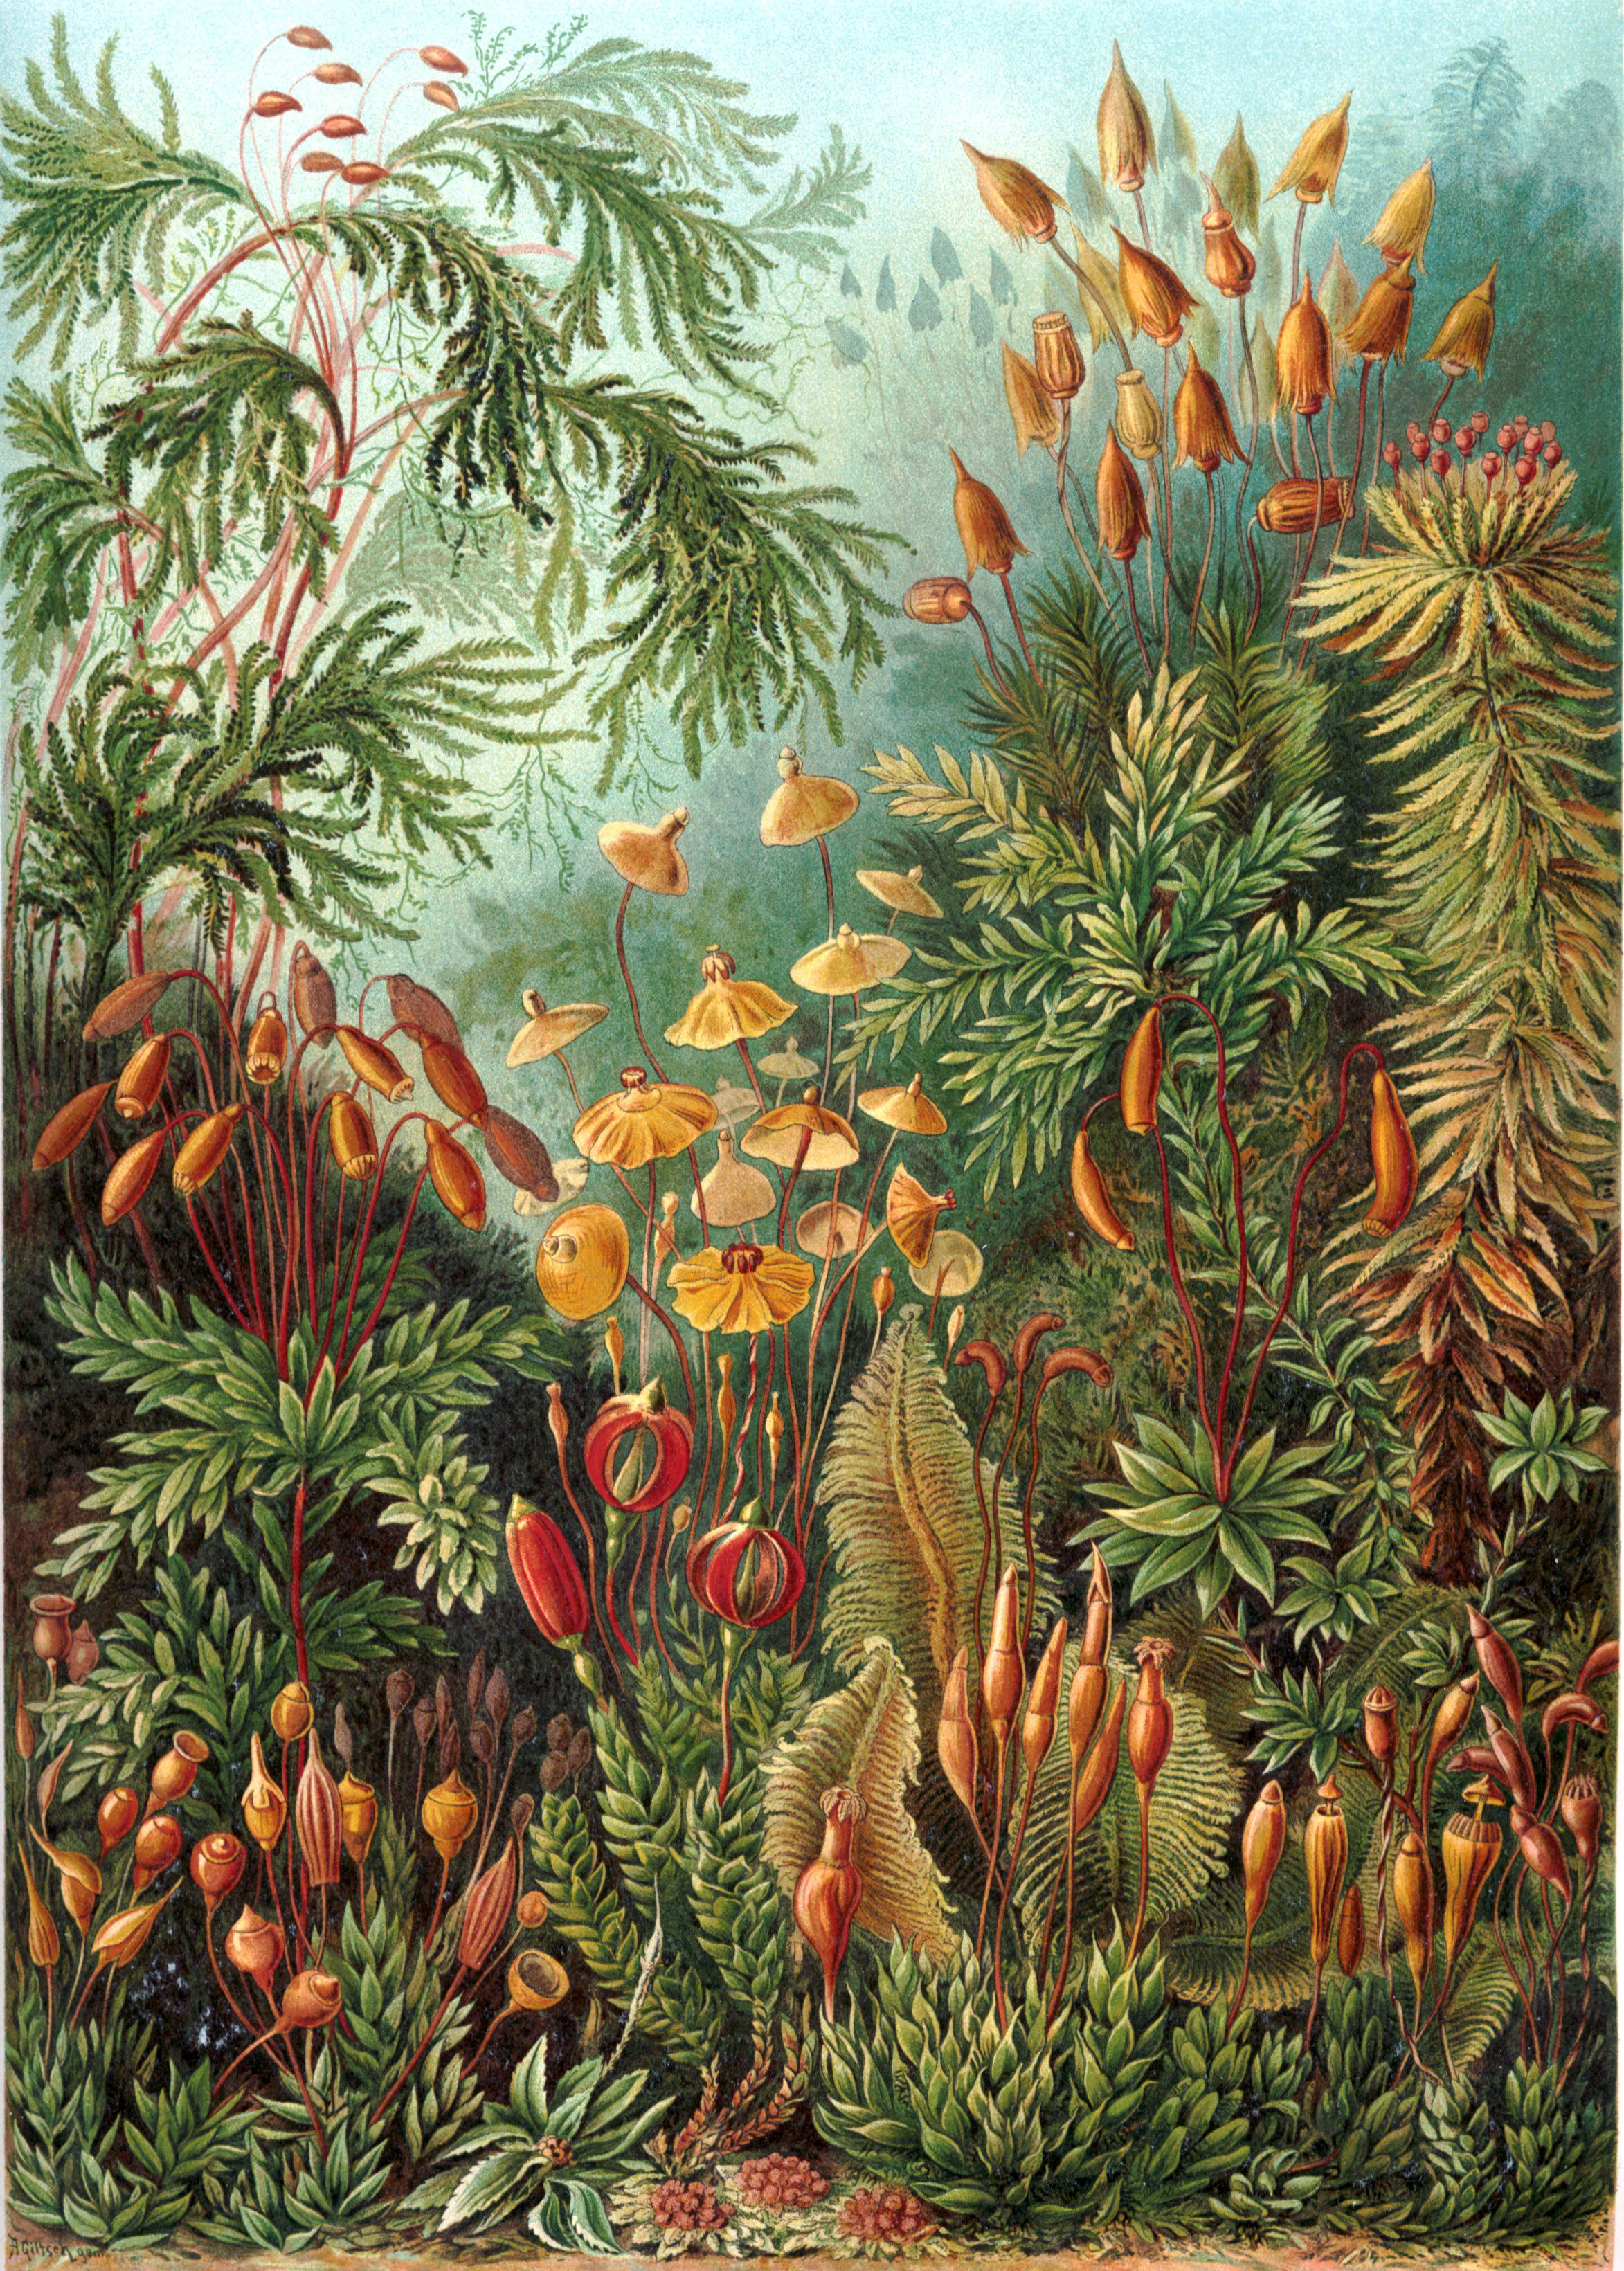
\includegraphics[width=0.7\linewidth]{./figures/mosses/Haeckel_Muscinae}

}

\caption{\href{https://commons.wikimedia.org/wiki/File:Haeckel_Muscinae.jpg}{Mosses}
from Ernst Haeckel's
\href{https://en.wikipedia.org/wiki/Kunstformen_der_Natur}{Kunstformen
der Natur}, 1904.}\label{fig:mosses}
\end{figure}

\subsection{Life cycle}\label{life-cycle}

The moss life-cycle (Figure \ref{fig:moss}) starts with a haploid spore
that germinates to produce a protonema (pl. protonemata), which is
either a mass of thread-like filaments or thalloid (flat and
thallus-like). Massed moss protonemata typically look like a thin green
felt, and may grow on damp soil, tree bark, rocks, concrete, or almost
any other reasonably stable surface. This is a transitory stage in the
life of a moss, but from the protonema grows the gametophyte that is
structurally differentiated into stems and leaves. A single mat of
protonemata may develop several gametophore shoots, resulting in a clump
of moss. From the tips of the gametophyte stems or branches develop the
sex organs of the mosses. The female organs are known as archegonia
(sing. archegonium) and are protected by a group of modified leaves
known as the perichaetum (plural, perichaeta). The archegonia are small
flask-shaped clumps of cells with an open neck (venter) down which the
male sperm swim. The male organs are known as antheridia (sing.
antheridium) and are enclosed by modified leaves called the perigonium
(pl. perigonia). The surrounding leaves in some mosses form a splash
cup, allowing the sperm contained in the cup to be splashed to
neighboring stalks by falling water droplets. In the presence of water,
sperm from the antheridia swim to the archegonia and fertilization
occurs, leading to the production of a diploid sporophyte. The sperm of
mosses is biflagellate, i.e.~they have two flagellae that aid in
propulsion. Since the sperm must swim to the archegonium, fertilization
cannot occur without water. Some species (for example \emph{Mnium hornum} or
several species of \emph{Polytrichum}) keep their antheridia in so called
`splash cups', bowl-like structures on the shoot tips that propel the
sperm several decimeters when water droplets hit it, increasing the
fertilization distance. After fertilization, the immature sporophyte
pushes its way out of the archegonial venter. It takes about a quarter
to half a year for the sporophyte to mature. The sporophyte body
comprises a long stalk, called a seta, and a capsule capped by a cap
called the operculum. The capsule and operculum are in turn sheathed by
a haploid calyptra which is the remains of the archegonial venter. The
calyptra usually falls off when the capsule is mature. Within the
capsule, spore-producing cells undergo meiosis to form haploid spores,
upon which the cycle can start again. The mouth of the capsule is
usually ringed by a set of teeth called peristome. Most mosses rely on
the wind to disperse the spores.

\begin{figure}

{\centering 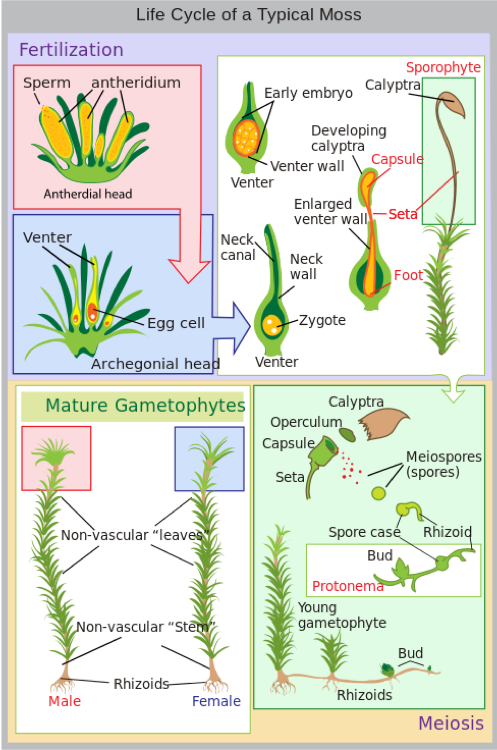
\includegraphics[width=0.7\linewidth]{./figures/mosses/moss_life_cycle}

}

\caption{\href{https://commons.wikimedia.org/wiki/File:Lifecycle_moss_svg_diagram.svg}{Life
cycle of mosses.}}\label{fig:moss}
\end{figure}

\section{View Prepared Slides of
Mosses}\label{view-the-prepared-slides-of-mosses}

\begin{enumerate}
\def\labelenumi{\arabic{enumi}.}
\tightlist
\item
  Moss archegonium (Figure \ref{fig:mossarchegonium})

  \begin{itemize}
  \tightlist
  \item
    Identify: female gametophyte tissue; archegonium with egg inside the
    venter
  \end{itemize}
\item
  Moss antheridium (Figure \ref{fig:mossantheridium})

  \begin{itemize}
  \tightlist
  \item
    Identify: male gametophyte tissue; antheridia with sperms inside;
    paraphyses (sterile filaments)
  \end{itemize}
\item
  Moss mature capsule (Figure \ref{fig:mosscapsule})

  \begin{itemize}
  \tightlist
  \item
    Identify: capsule; spores; operculum (cap); seta
  \end{itemize}
\item
  Moss protonema with bulbs w.m.

  \begin{itemize}
  \tightlist
  \item
    Identify: protonema filaments; gametophyte bulbs
  \end{itemize}
\end{enumerate}

\begin{figure}

{\centering 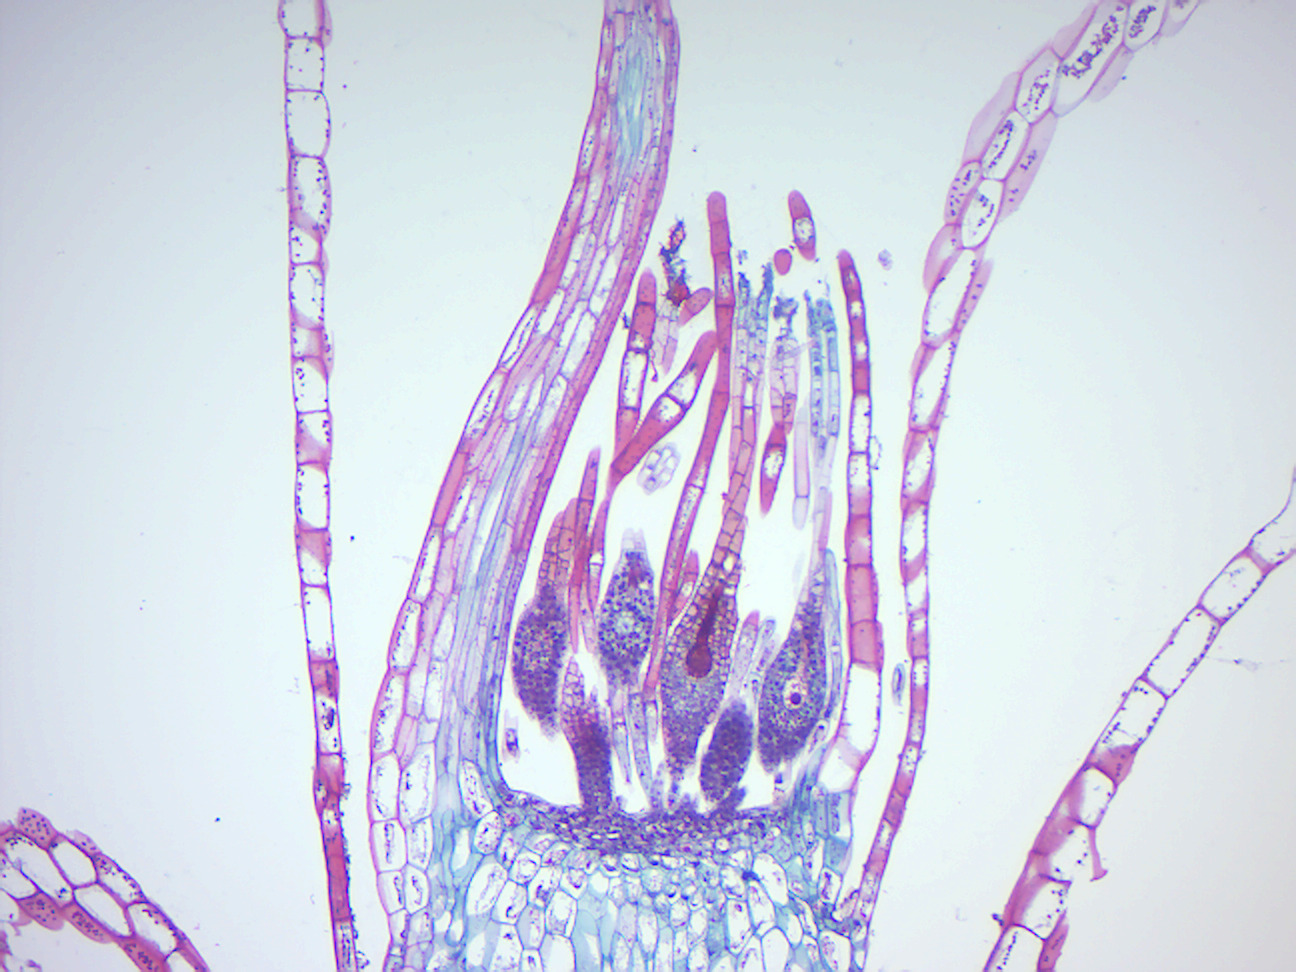
\includegraphics[width=0.7\linewidth]{./figures/mosses/moss_archegonium}

}

\caption{Moss archegonium.}\label{fig:mossarchegonium}
\end{figure}

\begin{figure}

{\centering 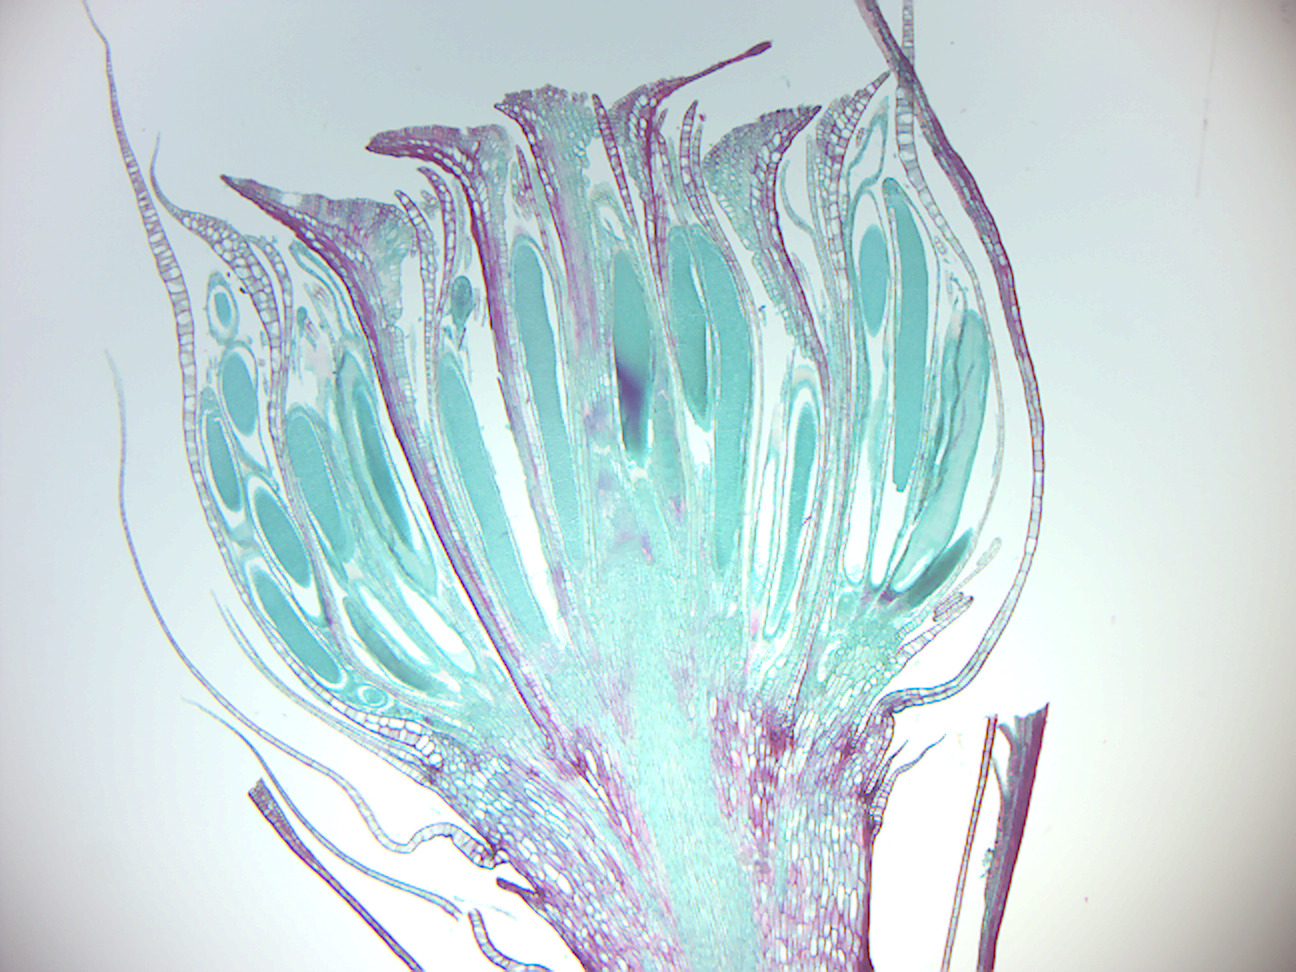
\includegraphics[width=0.7\linewidth]{./figures/mosses/moss_antheridium}

}

\caption{Moss antheridium.}\label{fig:mossantheridium}
\end{figure}

\begin{figure}

{\centering 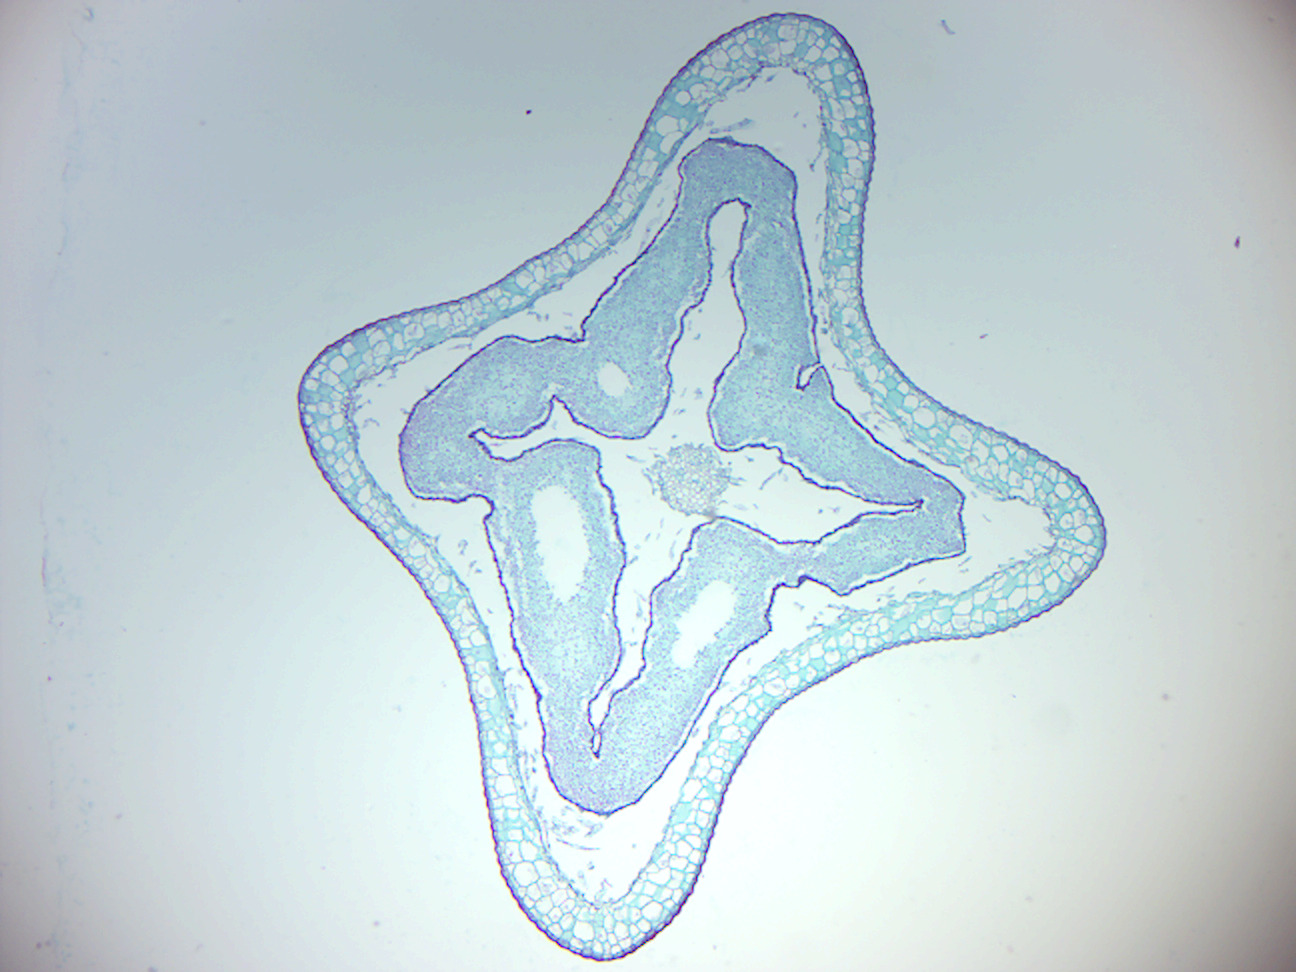
\includegraphics[width=0.7\linewidth]{./figures/mosses/moss_capsule}

}

\caption{Moss mature capsule.}\label{fig:mosscapsule}
\end{figure}

\section{Liverworts}\label{liverworts}

The
\href{https://en.wikipedia.org/wiki/Marchantiophyta}{Marchantiophyta}
(\href{https://commons.wikimedia.org/wiki/File:Haeckel_Hepaticae.jpg}{Figure
\ref{fig:hepatica}}) are a division of non-vascular land plants commonly
referred to as hepatics or liverworts. Like mosses and hornworts, they
have a gametophyte-dominant life cycle, in which cells of the plant
carry only a single set of genetic information. It is estimated that
there are about 9000 species of liverworts. Some of the more familiar
species grow as a flattened leafless thallus, but most species are leafy
with a form very much like a flattened moss. Liverworts are typically
small, usually from 2--20 mm wide with individual plants less than 10 cm
long, and are therefore often overlooked. However, certain species may
cover large patches of ground, rocks, trees or any other reasonably firm
substrate on which they occur. They are distributed globally in almost
every available habitat, most often in humid locations although there
are desert and Arctic species as well. Some species can be a nuisance in
shady greenhouses or a weed in gardens.

\begin{figure}

{\centering 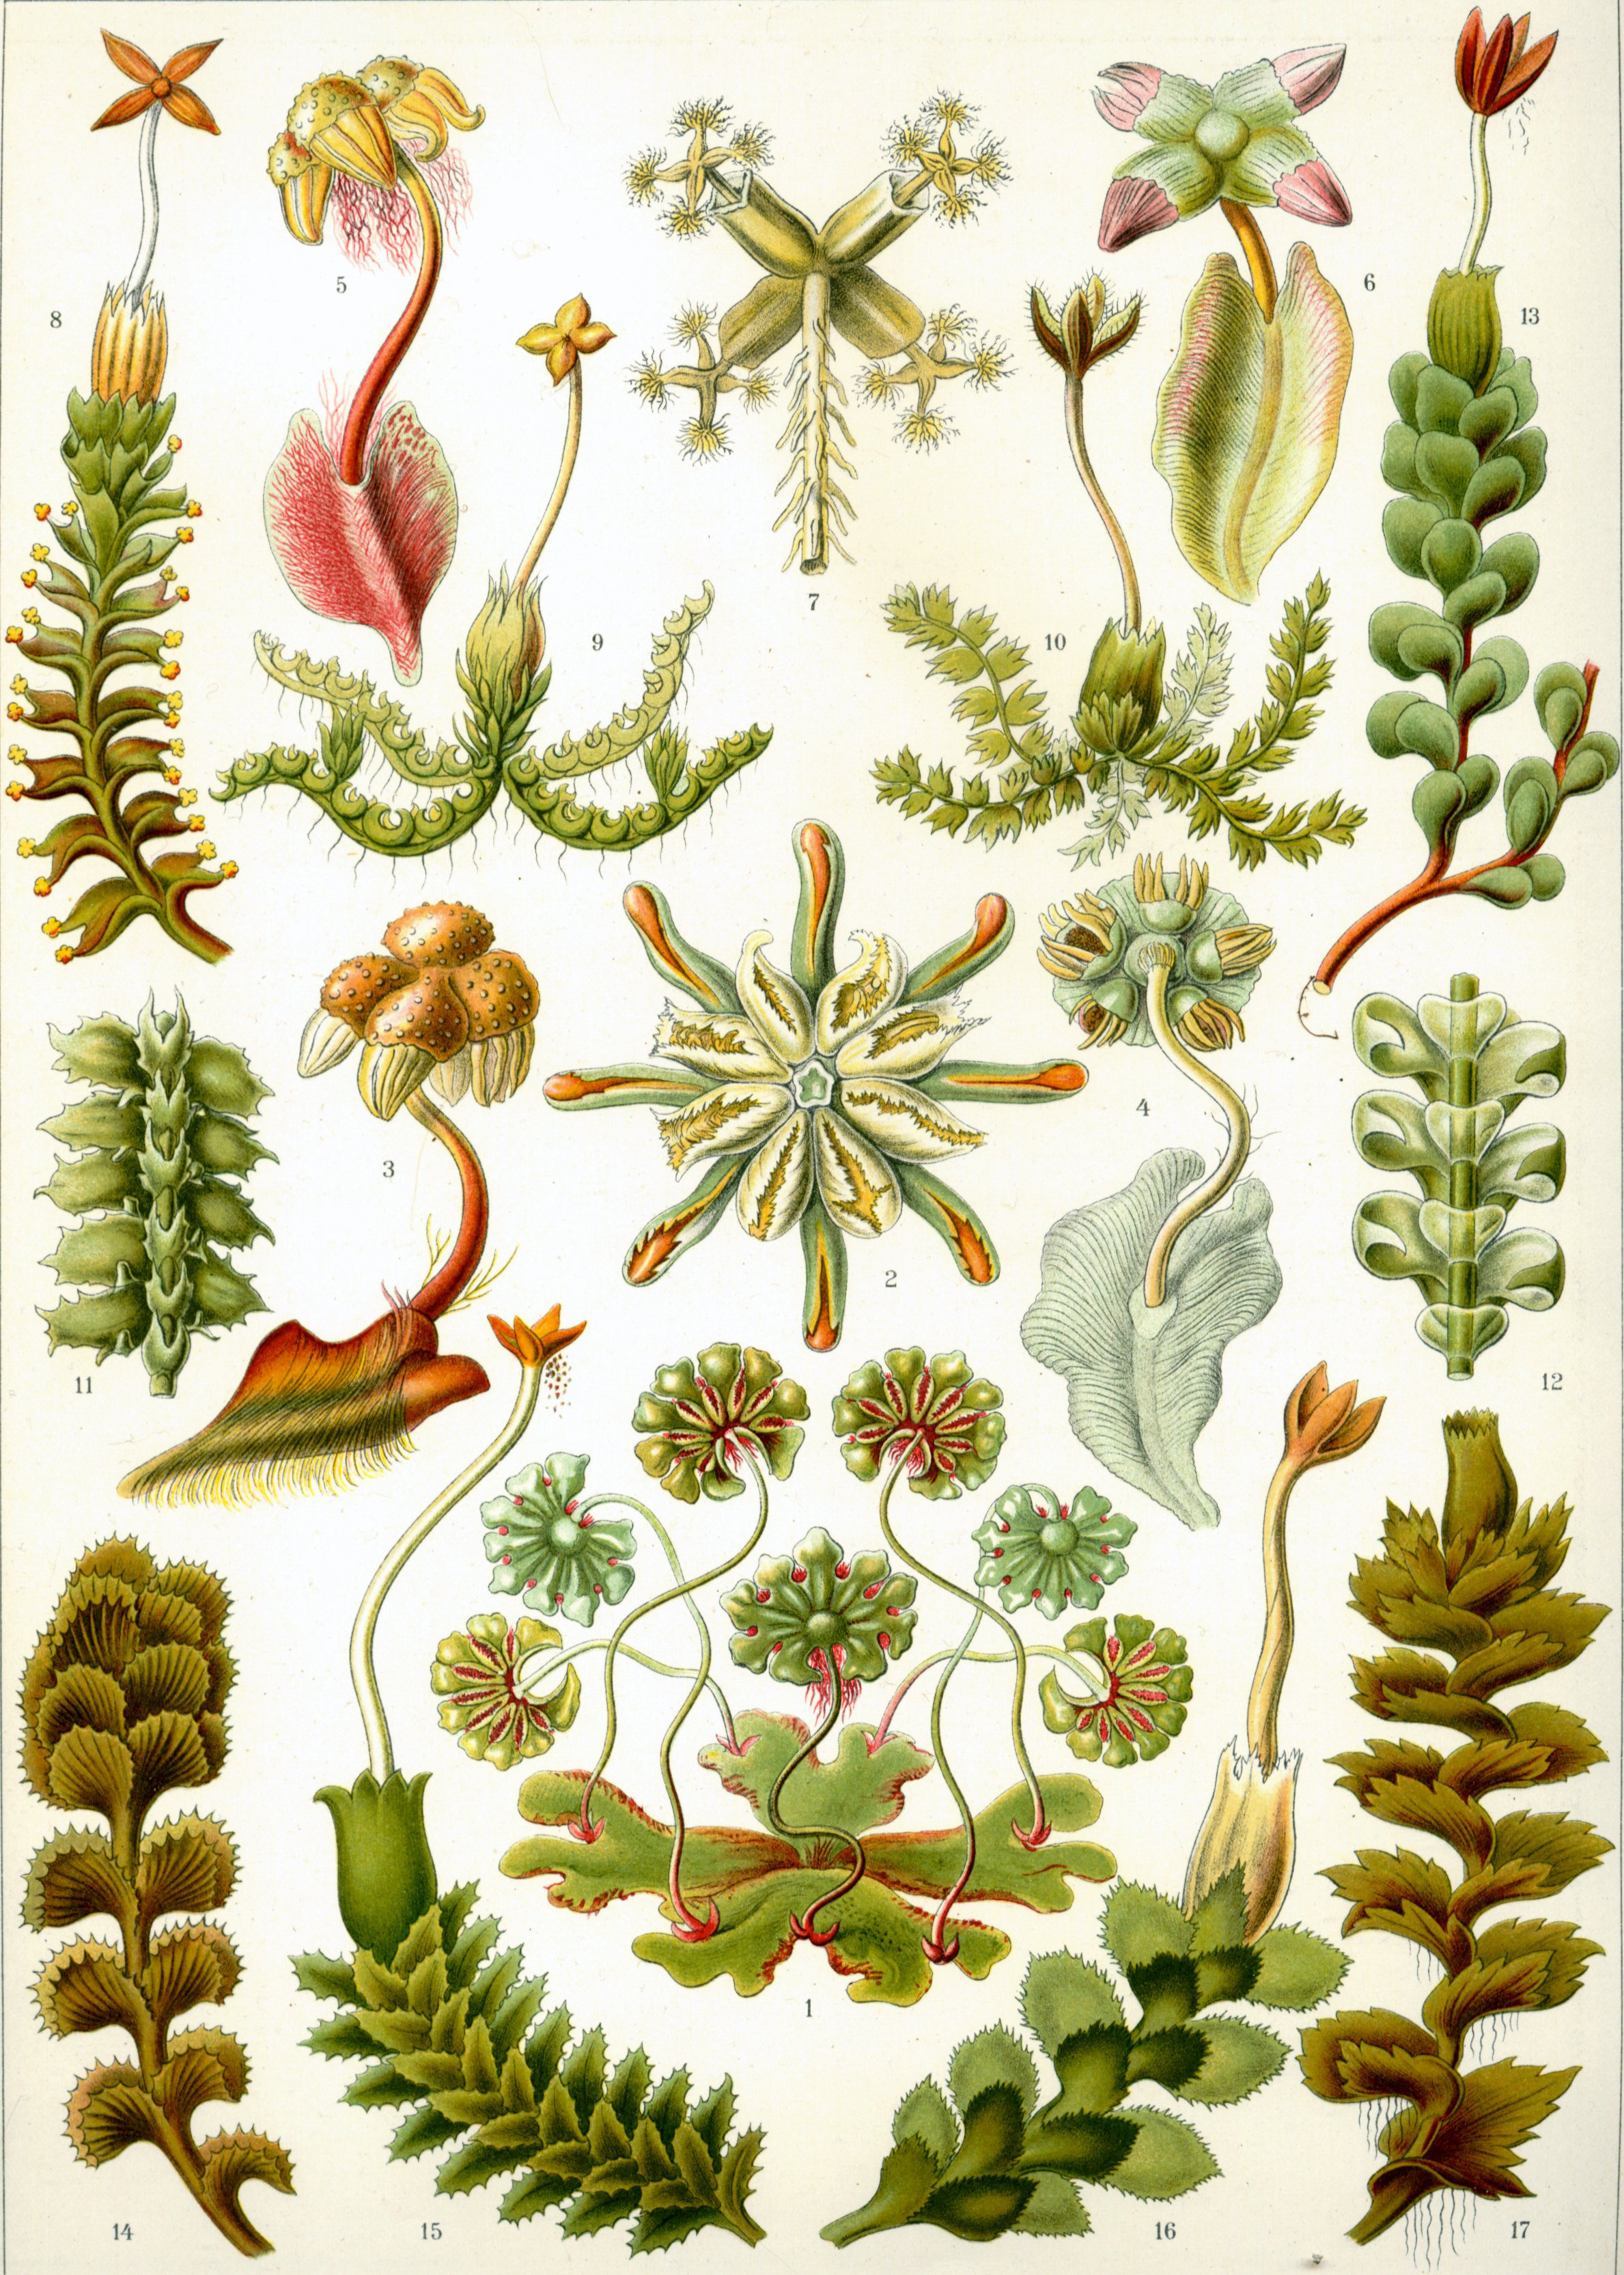
\includegraphics[width=0.7\linewidth]{./figures/mosses/Haeckel_Hepaticae}

}

\caption{\href{https://commons.wikimedia.org/wiki/File:Haeckel_Hepaticae.jpg}{Liverworts}
from Ernst Haeckel's
\href{https://en.wikipedia.org/wiki/Kunstformen_der_Natur}{Kunstformen
der Natur}, 1904.}\label{fig:hepatica}
\end{figure}

\subsection{Life cycle}\label{life-cycle-1}

The life of a liverwort starts from the germination of a haploid spore
to produce a protonema, which is either a mass of thread-like filaments
or else a flattened thallus. The protonema is a transitory stage in the
life of a liverwort, from which will grow the mature gametophyte plant
that produces the sex organs. The male organs are known as antheridia
(singular: antheridium) and produce the sperm cells. Clusters of
antheridia are enclosed by a protective layer of cells called the
perigonium (plural: perigonia). As in other land plants, the female
organs are known as archegonia (singular: archegonium) and are protected
by the thin surrounding perichaetum (plural: perichaeta). Each
archegonium has a slender hollow tube, the ``neck'', down which the
sperm swim to reach the egg cell. Liverwort species may be either
dioecious or monoecious. In dioecious liverworts, female and male sex
organs are borne on different and separate gametophyte plants. In
monoecious liverworts, the two kinds of reproductive structures are borne
on different branches of the same plant. In either case, the sperm must
move from the antheridia where they are produced to the archegonium
where the eggs are held. The sperm of liverworts is biflagellate,
i.e.~they have two tail-like flagellae that enable them to swim short
distances, provided that at least a thin film of water is present. Their
journey may be assisted by the splashing of raindrops. When sperm reach
the archegonia, fertilization occurs, leading to the production of a
diploid sporophyte. After fertilization, the immature sporophyte within
the archegonium develops three distinct regions: (1) a foot, which both
anchors the sporophyte in place and receives nutrients from its
``mother'' plant, (2) a spherical or ellipsoidal capsule, inside which
the spores will be produced for dispersing to new locations, and (3) a
seta (stalk) which lies between the other two regions and connects them.
When the sporophyte has developed all three regions, the seta elongates,
pushing its way out of the archegonium and rupturing it. While the foot
remains anchored within the parent plant, the capsule is forced out by
the seta and is extended away from the plant and into the air. Within
the capsule, cells divide to produce both elater cells and
spore-producing cells. The elaters are spring-like, and will push open
the wall of the capsule to scatter themselves when the capsule bursts.
The spore-producing cells will undergo meiosis to form haploid spores to
disperse, upon which point the life cycle can start again. Some
liverworts are capable of asexual reproduction. Some thallose liverworts
such as \emph{Marchantia polymorpha} produce small disc-shaped gemmae in
shallow cups. \emph{Marchantia} gemmae can be dispersed up to 120 cm by rain
splashing into the cups.

\begin{figure}

{\centering 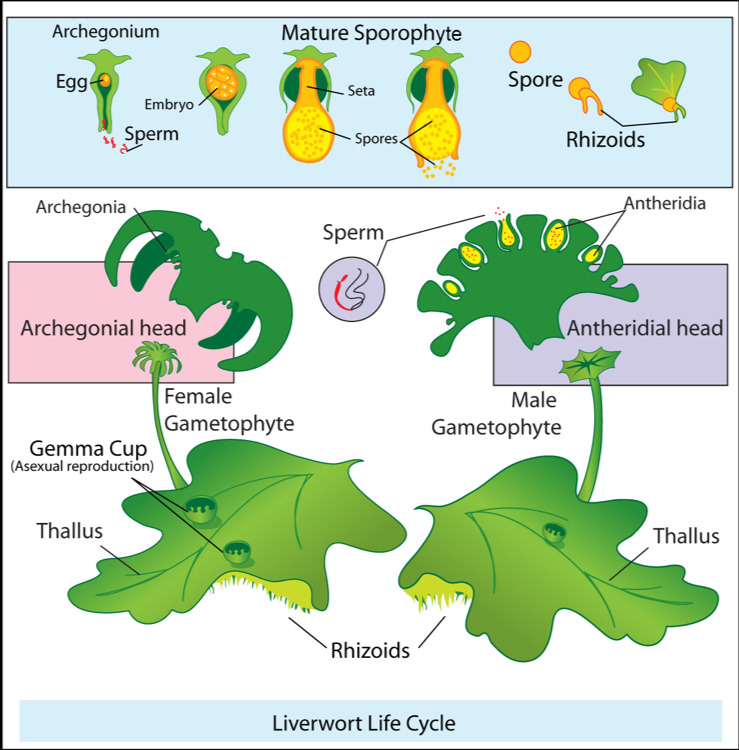
\includegraphics[width=0.7\linewidth]{./figures/mosses/liverwort_life_cycle}

}

\caption{\href{https://commons.wikimedia.org/wiki/File:Liverwort_life_cycle.jpg}{Life
cycle of liverworts.}
}\label{fig:liverwort}
\end{figure}

\section{View Prepared Slides of
Liverworts}\label{view-prepared-slides-of-liverworts}

\begin{enumerate}
\def\labelenumi{\arabic{enumi}.}
\tightlist
\item
  \emph{Marchantia} life history
\item
  \emph{Marchantia} thallus (Figure \ref{fig:marchantiathallus})

  \begin{itemize}
  \tightlist
  \item
    Identify: pores, tissue of lamina, rhizoids
  \end{itemize}
\item
  \emph{Marchantia} archegonia (Figure \ref{fig:marchantiaarchegonia})

  \begin{itemize}
  \tightlist
  \item
    Identify: archegonium with egg inside the venter; tissue of
    archegoniophore (female gametophyte)
  \end{itemize}
\item
  \emph{Marchantia} antheridia (Figure \ref{fig:marchantiaantheridia})

  \begin{itemize}
  \tightlist
  \item
    Identify: antheridia with sperms; tissue of antheridiophore (Male
    gametophyte); air chambers
  \end{itemize}
\item
  \emph{Marchantia} sporophyte (Figure \ref{fig:marchantiasporophyte})

  \begin{itemize}
  \tightlist
  \item
    Identify: sporophyte and its three parts: foot, seta (stalk), and
    capsule; spores and elaters inside the capsule; tissue of the female
    gametophyte
  \end{itemize}
\item
  \emph{Marchantia} gemma cup (Figure \ref{fig:gemma})

  \begin{itemize}
  \tightlist
  \item
    Identify: gemma cup and gemmae
  \end{itemize}
\end{enumerate}

\begin{figure}

{\centering 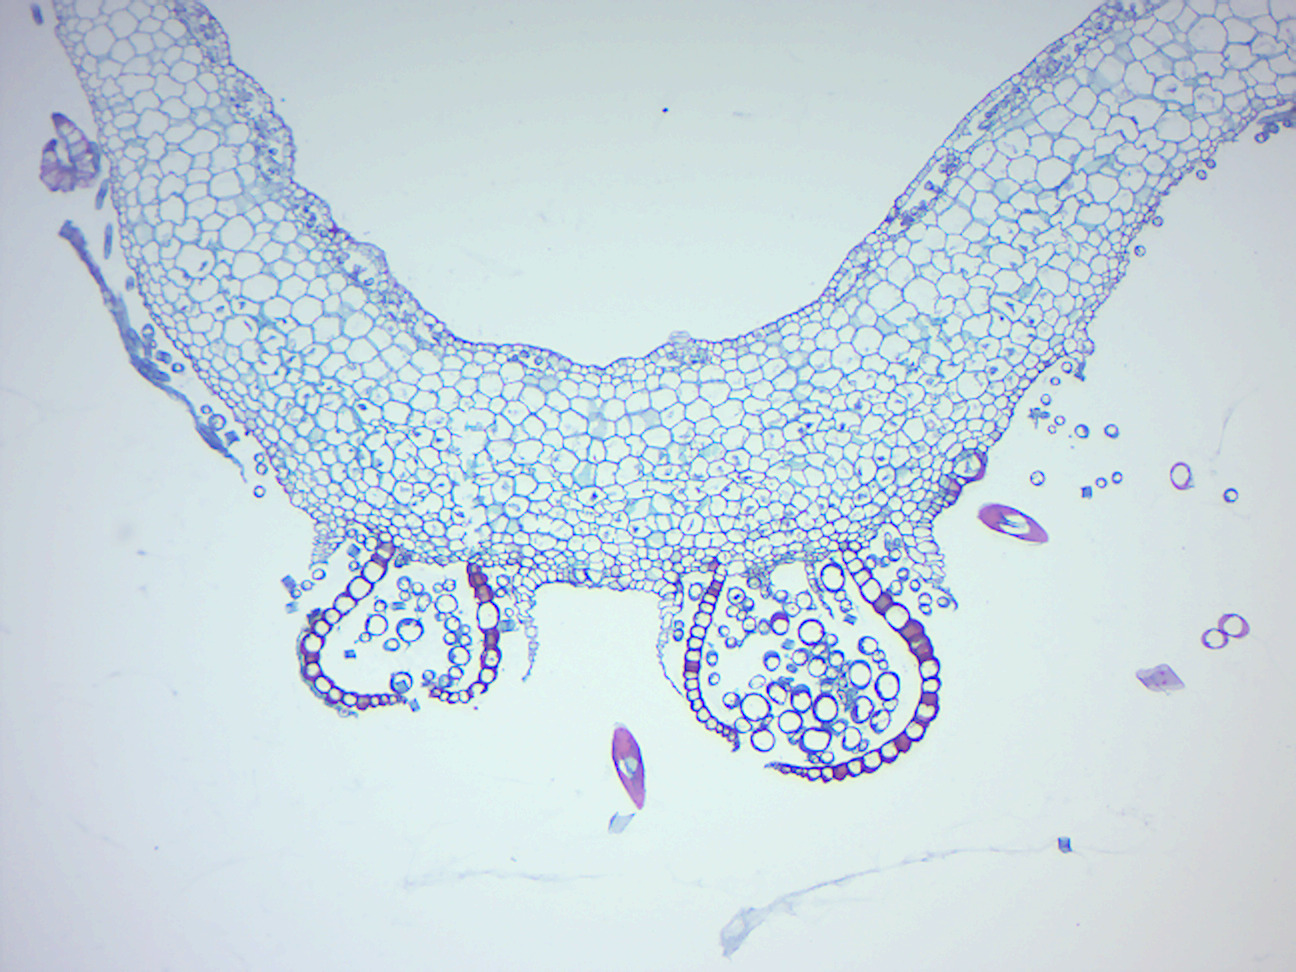
\includegraphics[width=0.7\linewidth]{./figures/mosses/marchantia_thallus}

}

\caption{\emph{Marchantia} thallus.}\label{fig:marchantiathallus}
\end{figure}

\begin{figure}

{\centering 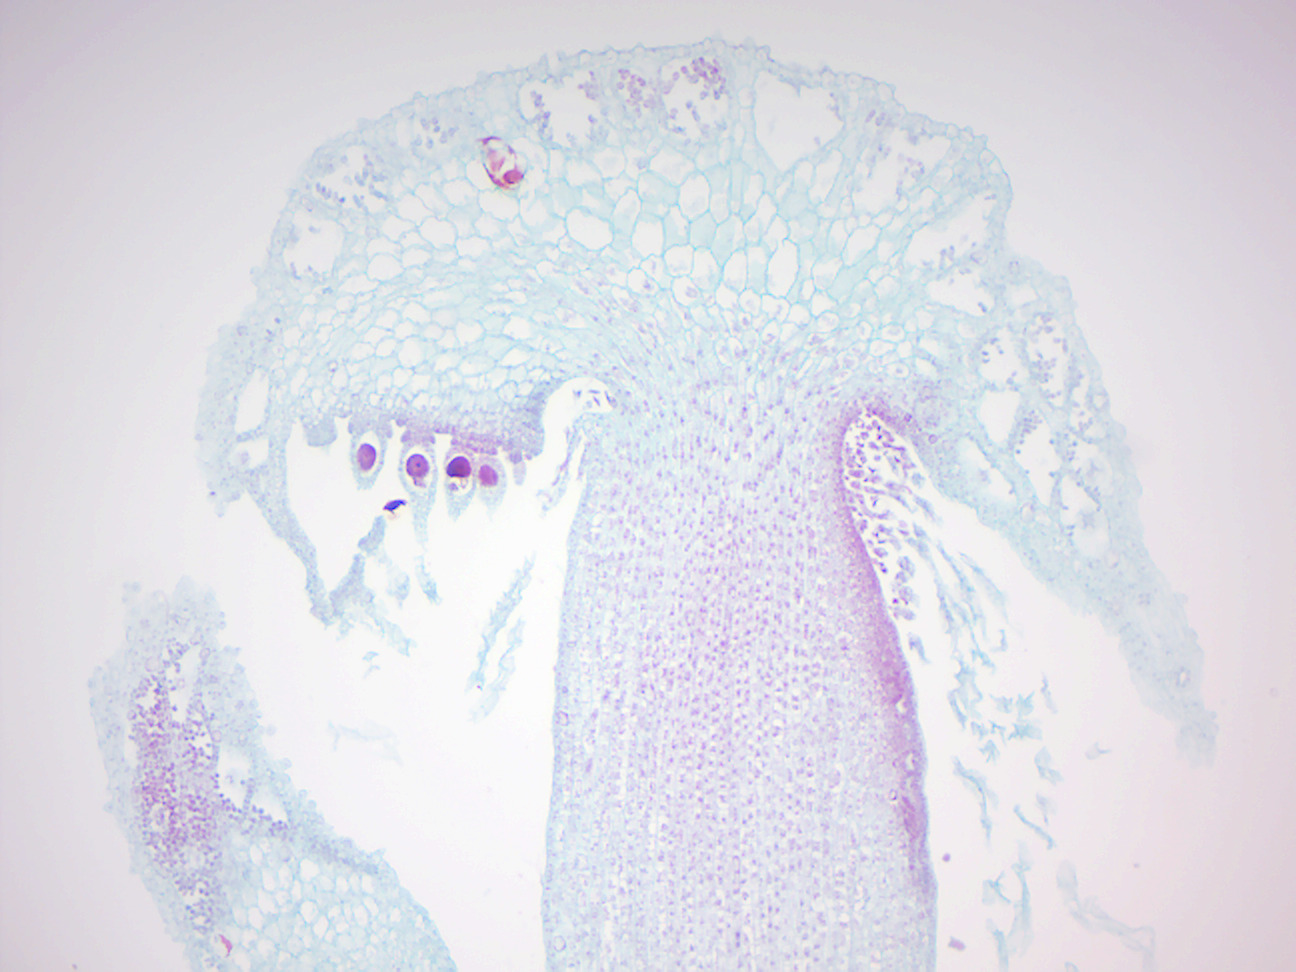
\includegraphics[width=0.7\linewidth]{./figures/mosses/marchantia_archegonia}

}

\caption{\emph{Marchantia} archegonia.}\label{fig:marchantiaarchegonia}
\end{figure}

\begin{figure}

{\centering 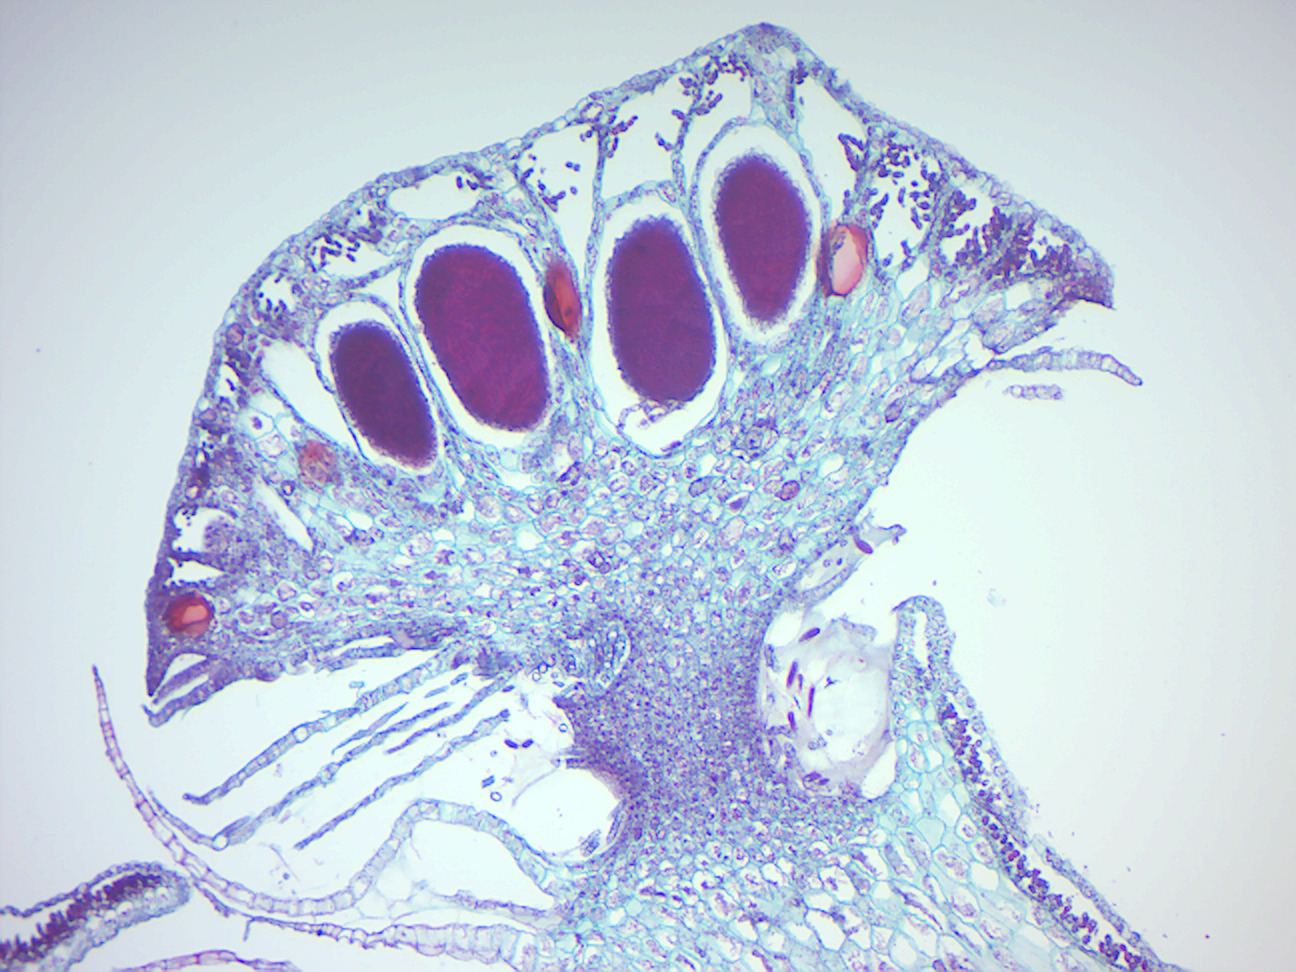
\includegraphics[width=0.7\linewidth]{./figures/mosses/marchantia_antheridia}

}

\caption{\emph{Marchantia} antheridia.}\label{fig:marchantiaantheridia}
\end{figure}

\begin{figure}

{\centering 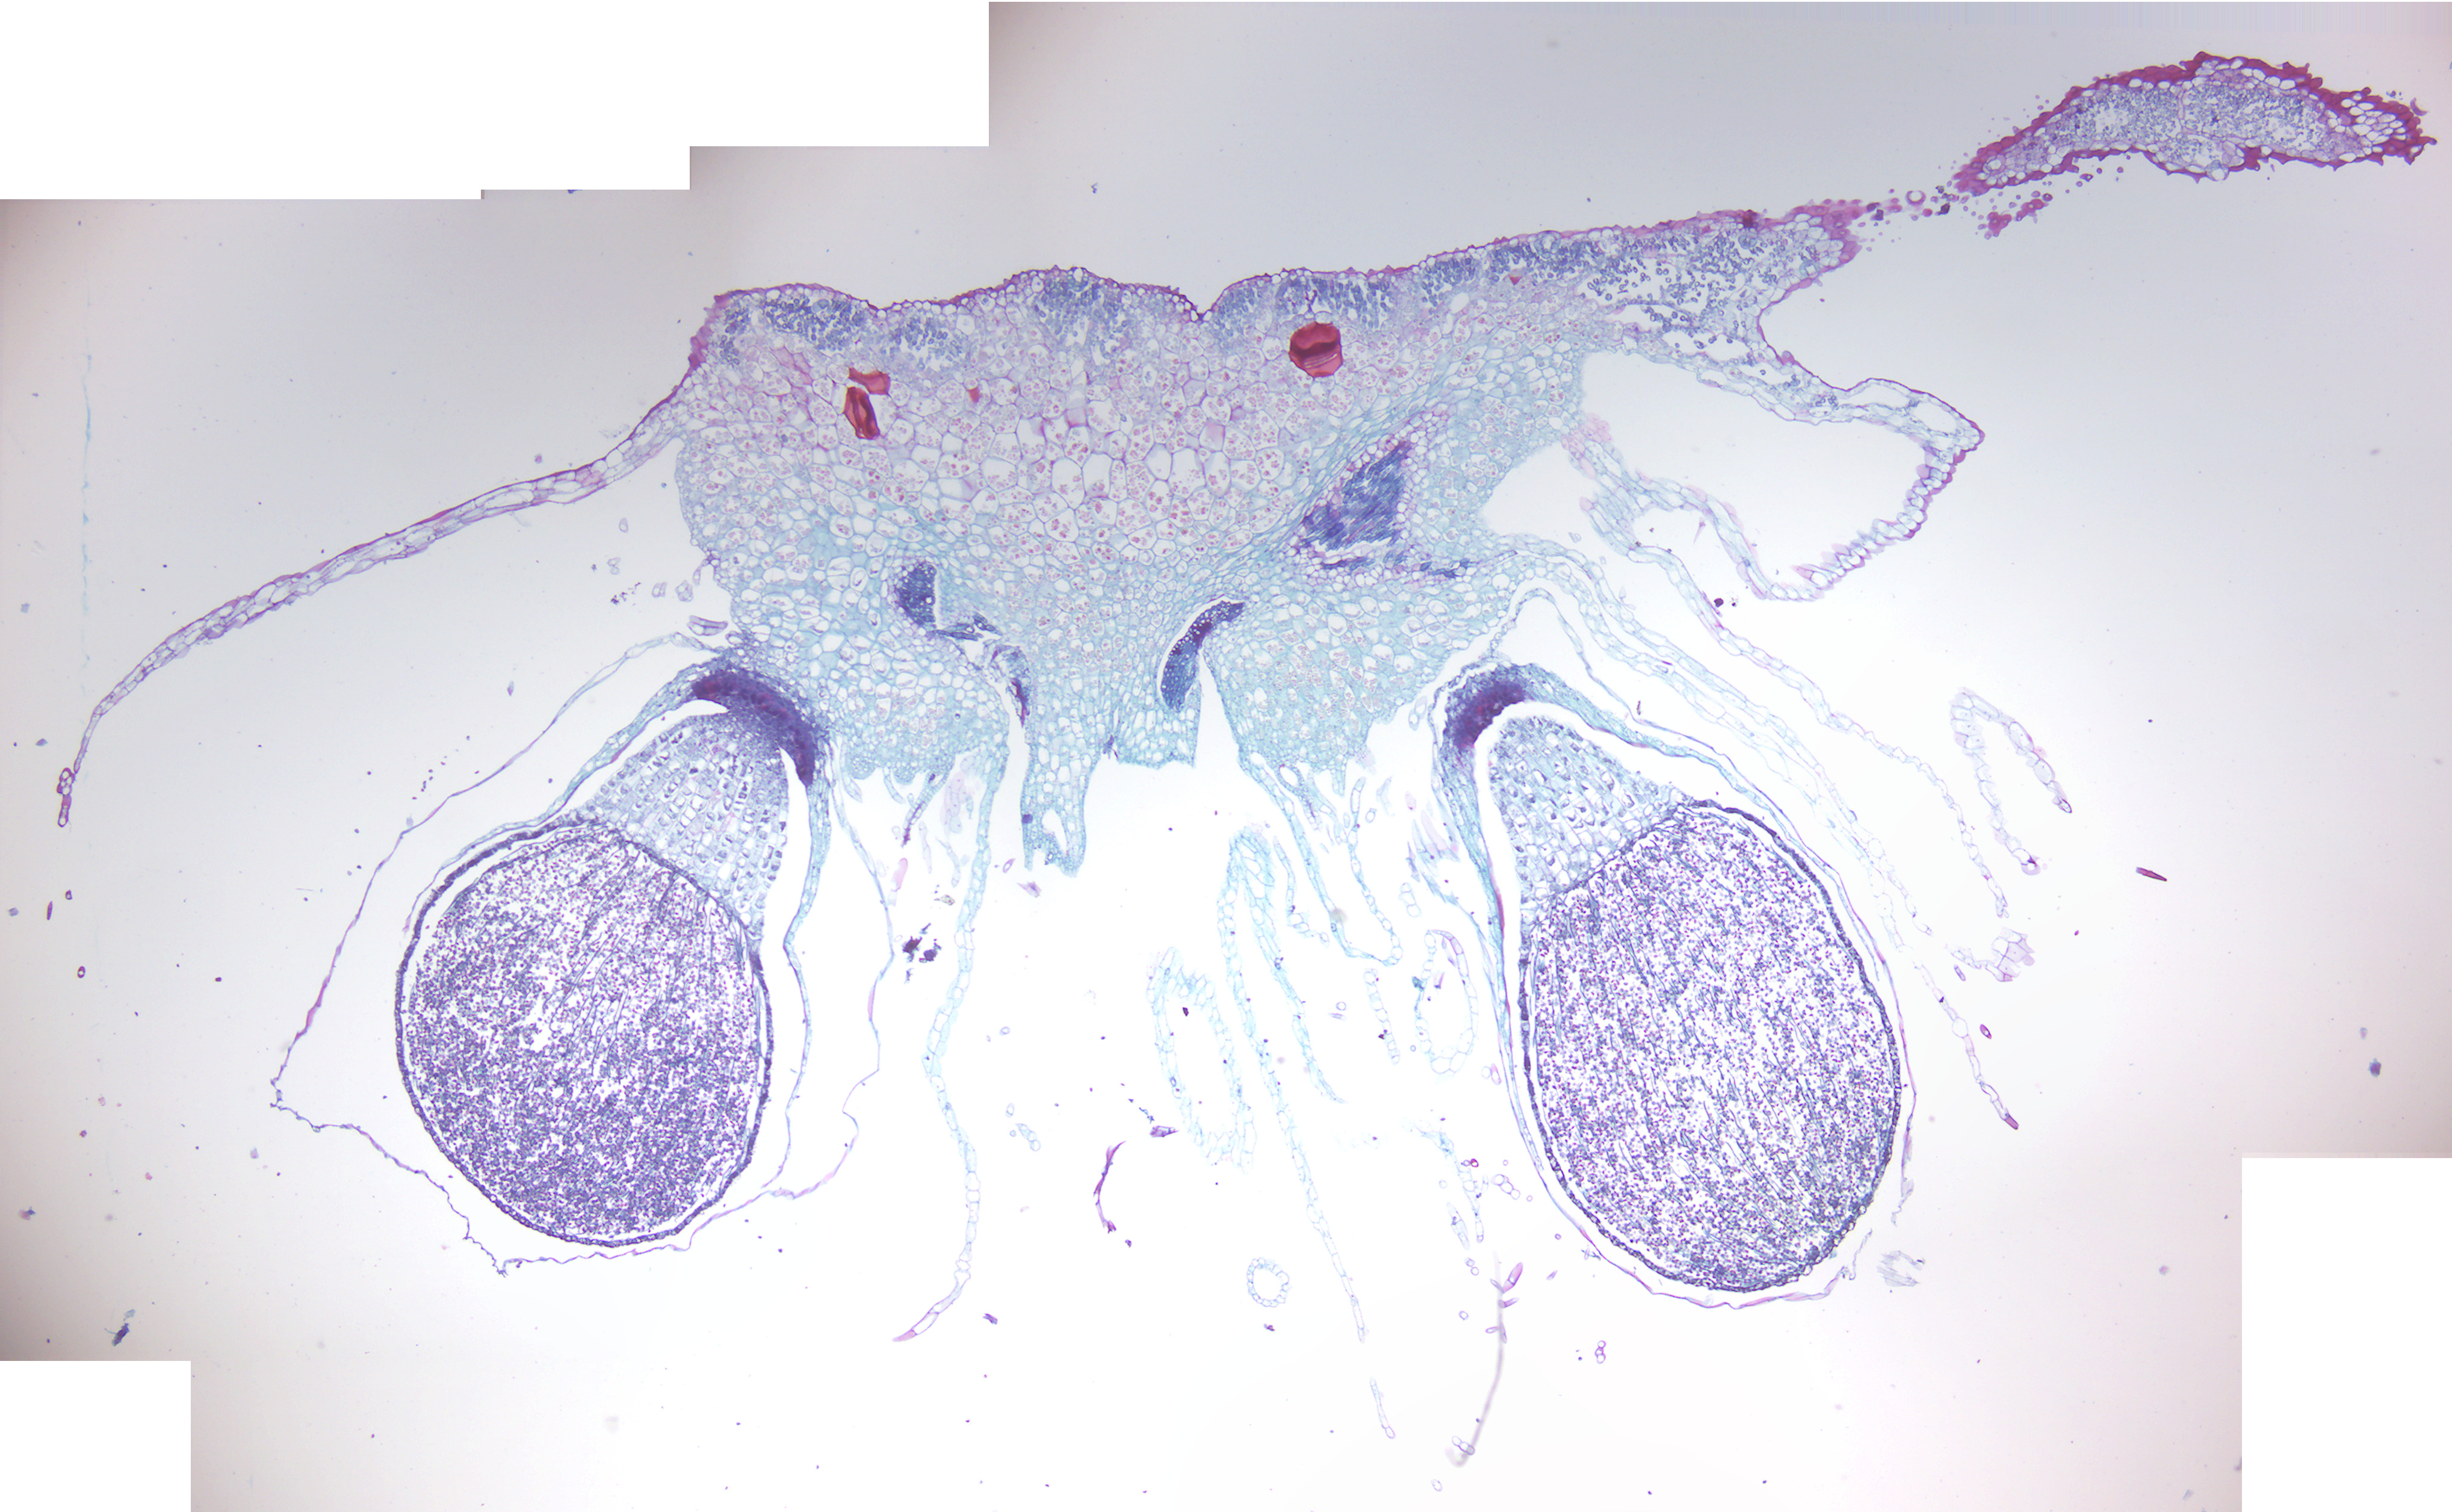
\includegraphics[width=0.7\linewidth]{./figures/mosses/marchantia_sporophyte}

}

\caption{\emph{Marchantia} sporophyte.}\label{fig:marchantiasporophyte}
\end{figure}

\begin{figure}

{\centering 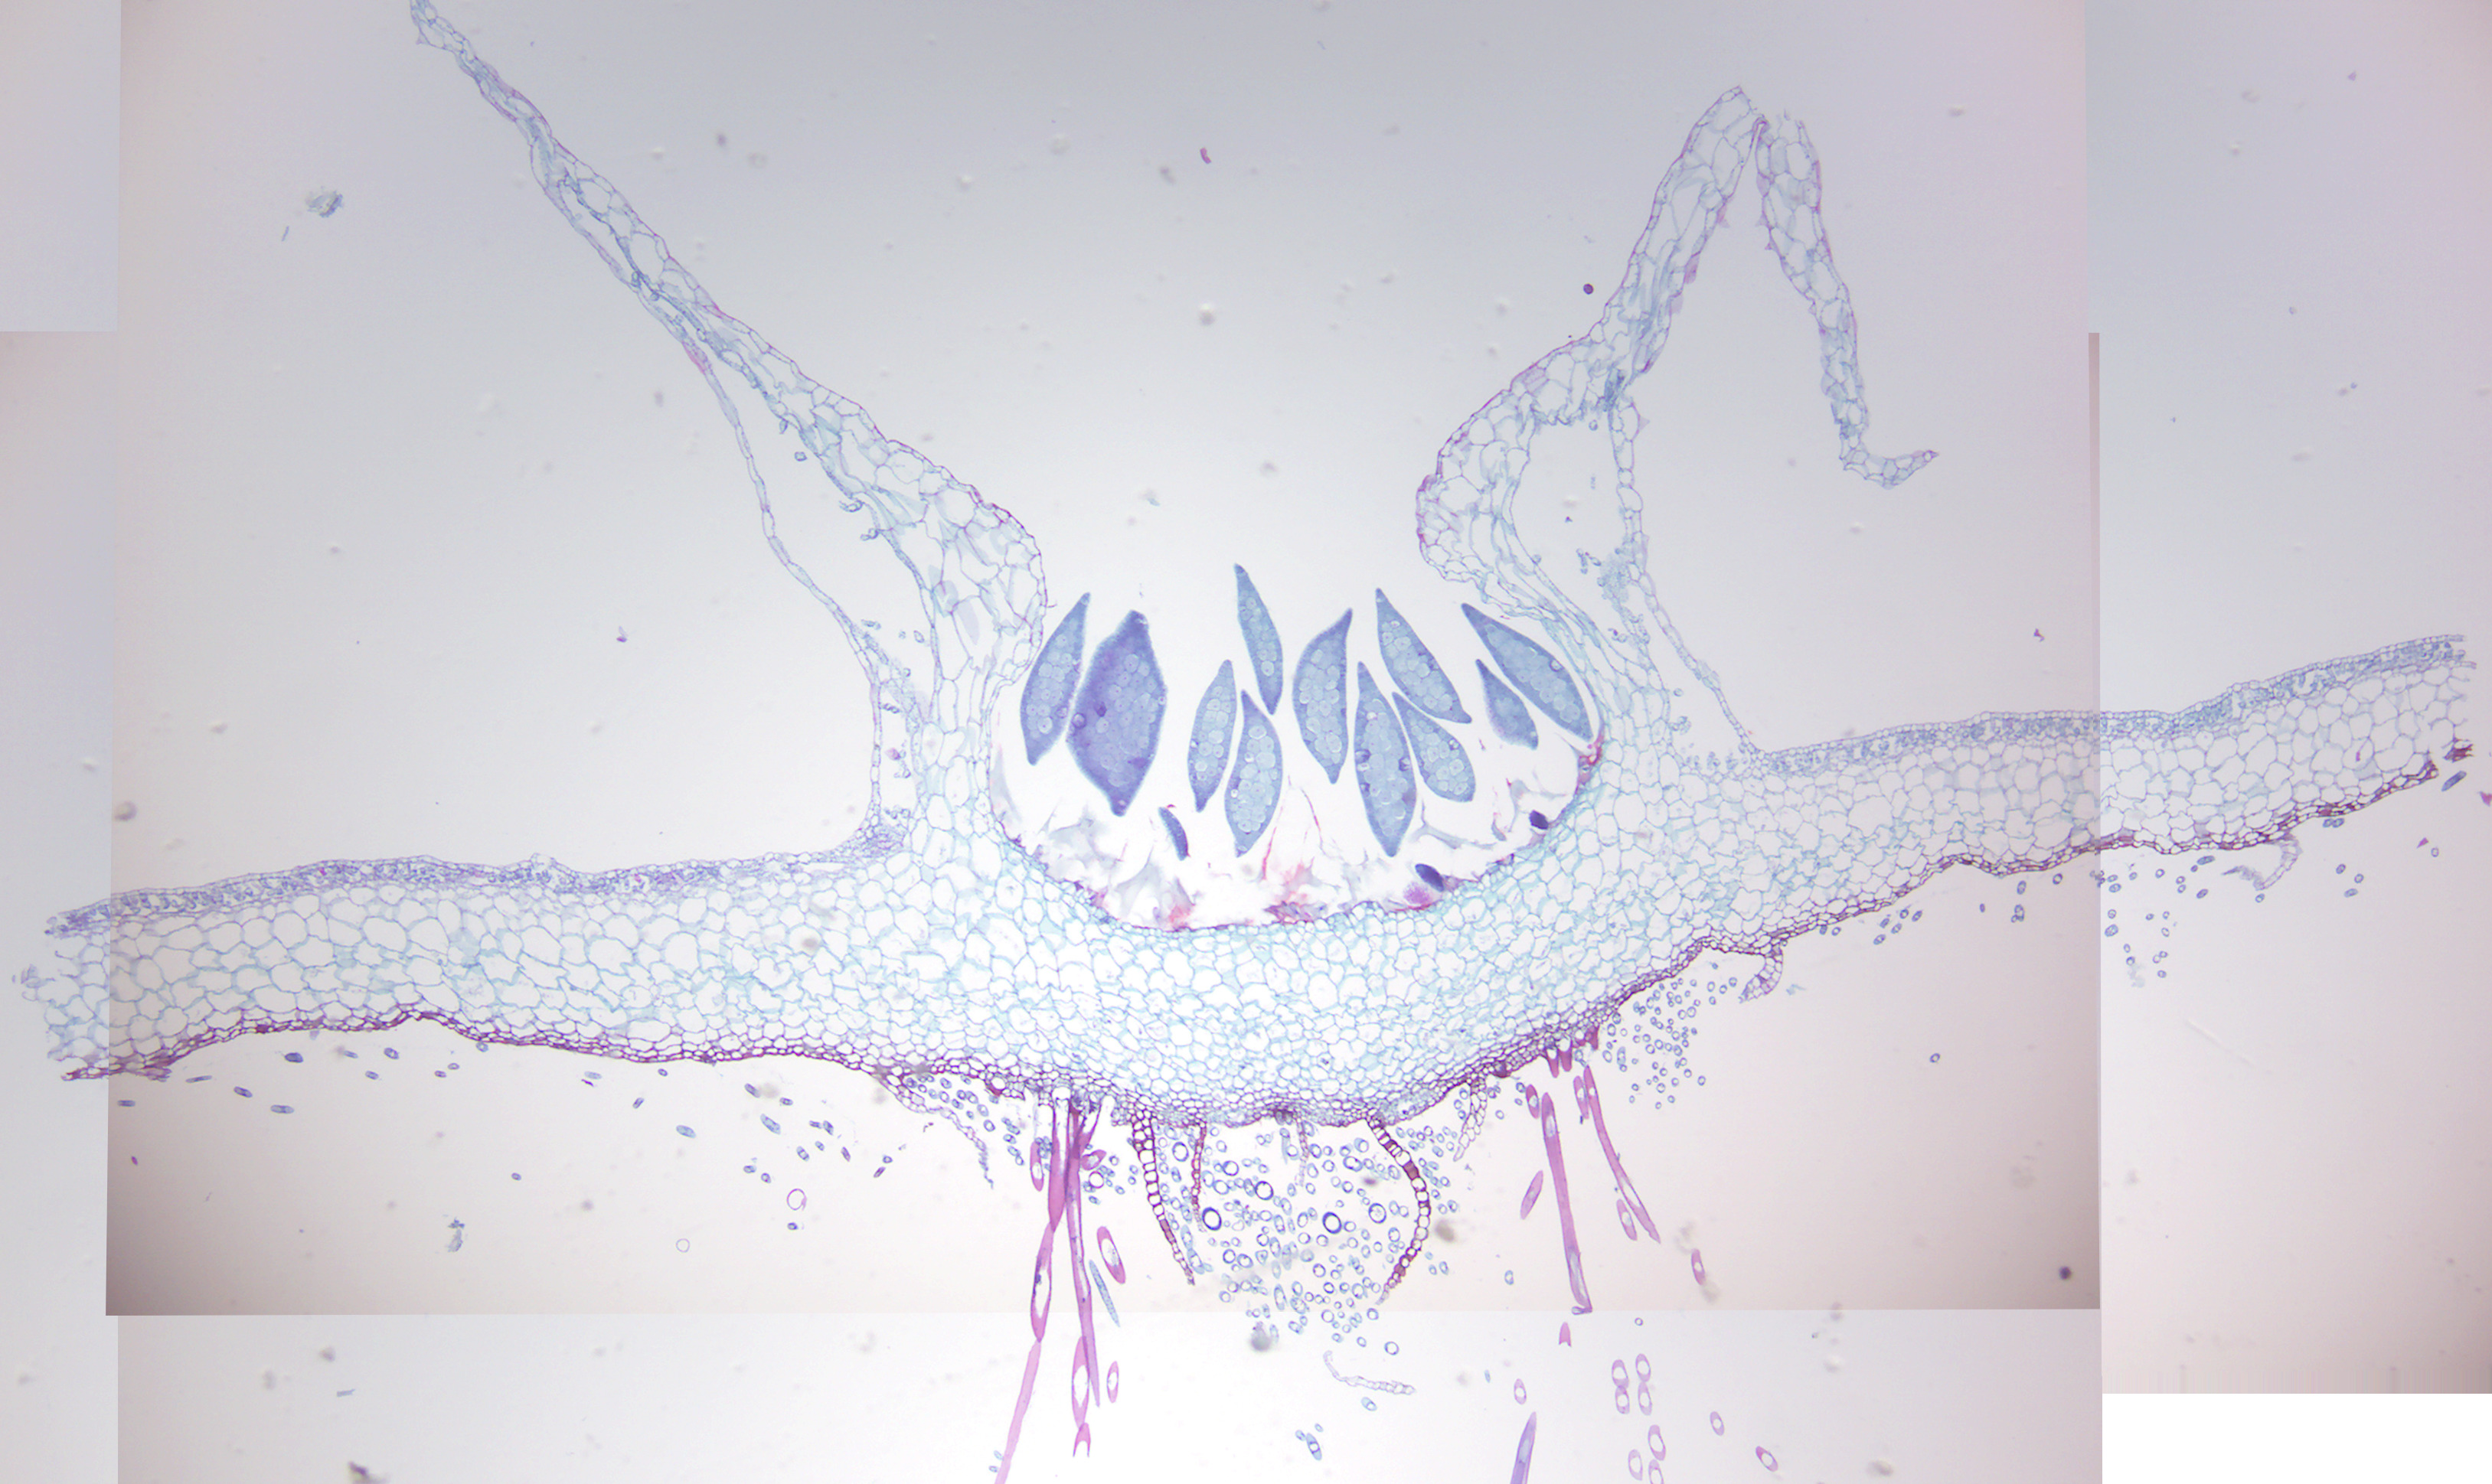
\includegraphics[width=0.7\linewidth]{./figures/mosses/marchantia_gemma_cup}

}

\caption{\emph{Marchantia} gemma cup.}\label{fig:gemma}
\end{figure}

\section{Vascular plants}\label{vascular-plants}

\href{https://en.wikipedia.org/wiki/Vascular_plant}{Vascular plants}
(from Latin vasculum: duct), also known as tracheophytes (from the
equivalent Greek term trachea) and also higher plants, form a large
group of plants (c. 308,312 accepted known species) that are defined as
those land plants that have lignified tissues (the xylem) for conducting
water and minerals throughout the plant. They also have a specialized
non-lignified tissue (the phloem) to conduct products of photosynthesis.
Vascular plants include the clubmosses, horsetails, ferns, gymnosperms
(including conifers) and angiosperms (flowering plants). Scientific
names for the group include Tracheophyta and Tracheobionta.

Vascular plants are distinguished by two primary characteristics:

\begin{enumerate}
\def\labelenumi{\arabic{enumi}.}
\tightlist
\item
  Vascular plants have vascular tissues which distribute resources
  through the plant. This feature allows vascular plants to evolve to a
  larger size than non-vascular plants, which lack these specialized
  conducting tissues and are therefore restricted to relatively small
  sizes.
\item
  In vascular plants, the principal generation phase is the sporophyte,
  which is usually diploid with two sets of chromosomes per cell. Only
  the germ cells and gametophytes are haploid. By contrast, the
  principal generation phase in non-vascular plants is the gametophyte,
  which is haploid with one set of chromosomes per cell. In these
  plants, only the spore stalk and capsule are diploid.
\end{enumerate}

Vascular plants first appeared during the Silurian period, and by the
Devonian had diversified and spread into many different terrestrial
environments. They developed a number of adaptations that allowed them
to spread into increasingly more arid places, notably the vascular
tissues xylem and phloem, that transport water and food throughout the
organism. Root systems capable of obtaining soil water and nutrients
also evolved during the Devonian. In modern vascular plants, the
sporophyte is typically large, branched, nutritionally independent and
long-lived, but there is increasing evidence that Paleozoic gametophytes
were just as complex as the sporophytes. The gametophytes of all
vascular plant groups evolved to become reduced in size and prominence
in the life cycle.

The first seed plants, pteridosperms (seed ferns), now extinct, appeared
in the Devonian and diversified through the Carboniferous. In these the
micro gametophyte is reduced to pollen and the mega gametophyte remains
inside the megasporangium, attached to the parent plant. A
megasporangium invested in protective layer called an integument is
known as an ovule. After fertilization by means of sperm deposited by
pollen grains, an embryo develops inside the ovule. The integument
becomes a seed coat, and the ovule develops into a seed. Seed plants can
survive and reproduce in extremely arid conditions, because they are not
dependent on free water for the movement of sperm, or the development of
free living gametophytes.

\section{Pteridophyta}\label{pteridophyta}

The \href{https://en.wikipedia.org/wiki/Pteridophyte}{pteridophytes} are
vascular plants (with xylem and phloem) that reproduce via spores, and
include the ferns, horsetails, and the lycophytes (clubmosses, spike
mosses, and quillworts). These are not a monophyletic group because
ferns and horsetails are more closely related to seed plants than to the
lycophytes. Therefore, ``Pteridophyta'' is now an invalid taxon,
although the term pteridophyte remains in common use.

\begin{figure}

{\centering 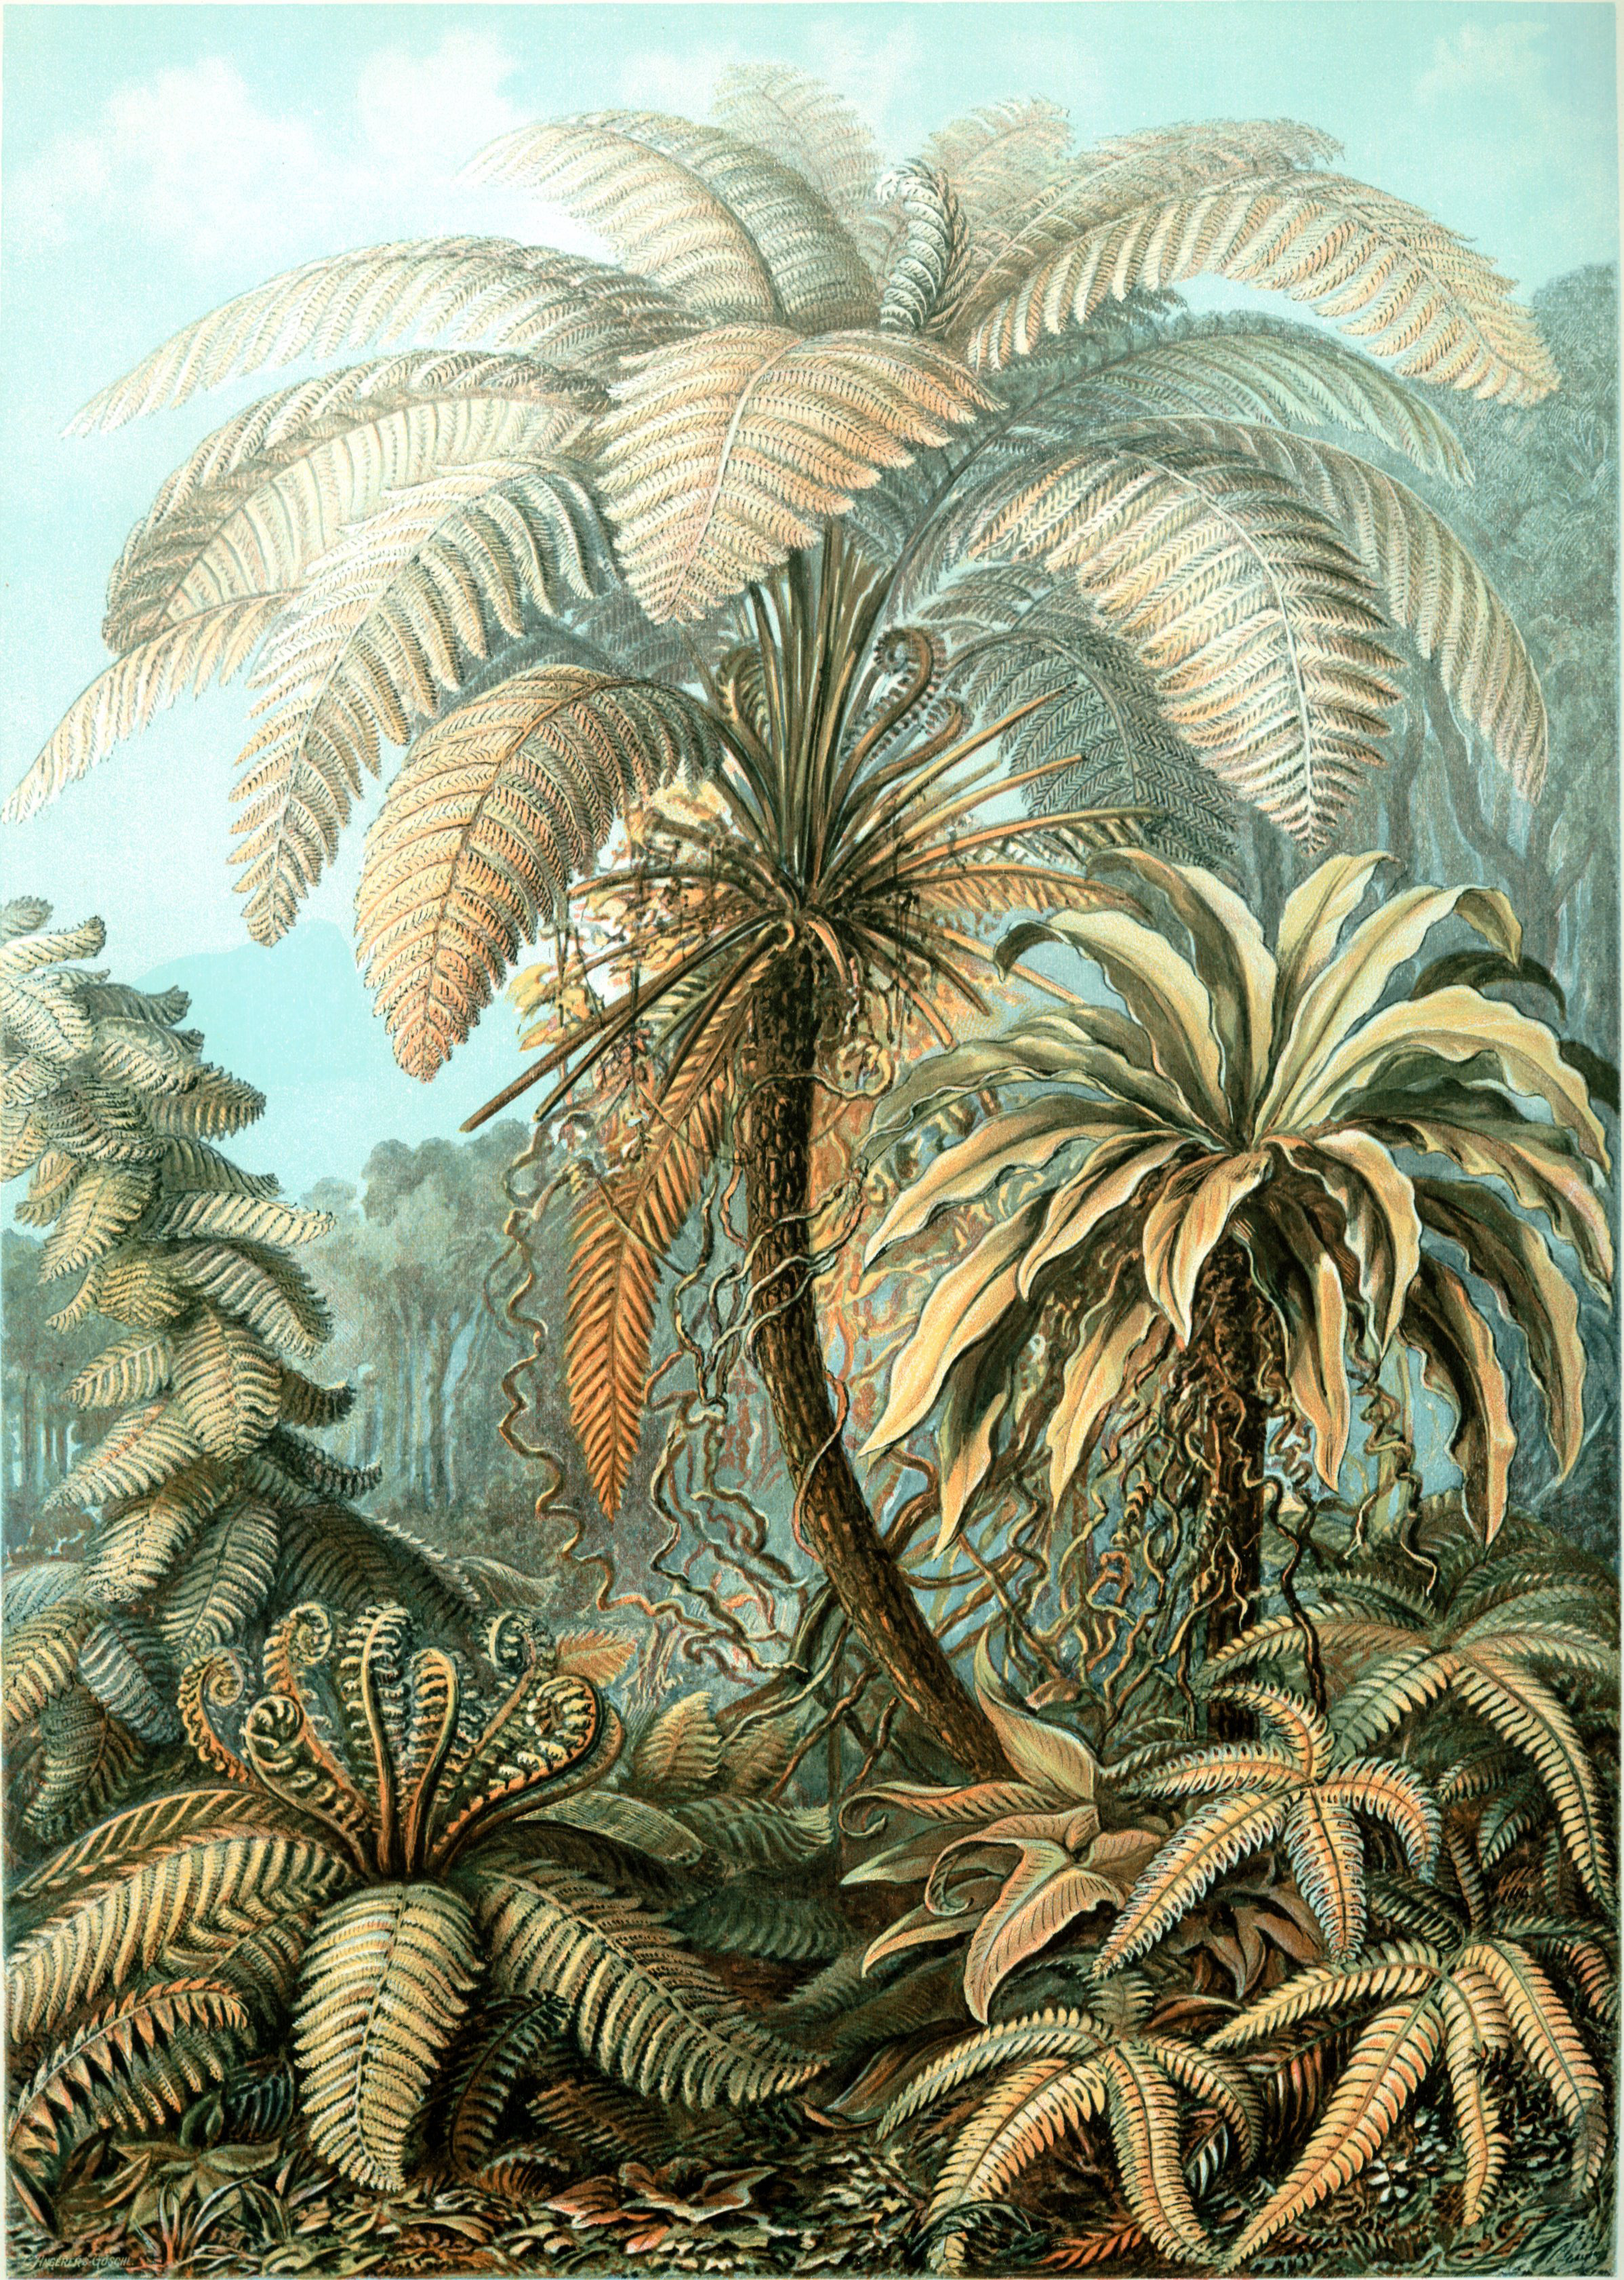
\includegraphics[width=0.7\linewidth]{./figures/mosses/Haeckel_Filicinae_92}

}

\caption{\href{https://commons.wikimedia.org/wiki/File:Haeckel_Filicinae_92.jpg}{Ferns}
from Ernst Haeckel's
\href{https://en.wikipedia.org/wiki/Kunstformen_der_Natur}{Kunstformen
der Natur}, 1904.}\label{fig:ferns}
\end{figure}

\subsection{Life cycle}\label{life-cycle-2}

Ferns are vascular plants differing from lycophytes by having true
leaves (megaphylls). They differ from seed plants (gymnosperms and
angiosperms) in their mode of reproduction---lacking flowers and seeds.
Like all land plants, they have a life cycle referred to as alternation
of generations, characterized by alternating diploid sporophytic and
haploid gametophytic phases. The diploid sporophyte has 2n paired
chromosomes, where n varies from species to species. The haploid
gametophyte has n unpaired chromosomes, i.e.~half the number of the
sporophyte. The gametophyte of ferns is a free-living organism, whereas
the gametophyte of the gymnosperms and angiosperms is dependent on the
sporophyte.

The life cycle of a typical fern proceeds as follows:

\begin{enumerate}
\def\labelenumi{\arabic{enumi}.}
\tightlist
\item
  A diploid sporophyte phase produces haploid spores by meiosis.
\item
  A spore grows into a haploid gametophyte by mitosis. The gametophyte
  typically consists of a photosynthetic prothallus.
\item
  The gametophyte produces gametes (often both sperm and eggs on the
  same prothallus) by mitosis.
\item
  A mobile, flagellate sperm fertilizes an egg that remains attached to
  the prothallus.
\item
  The fertilized egg is now a diploid zygote and grows by mitosis into a
  diploid sporophyte (the typical ``fern'' plant).
\end{enumerate}

\section{Clubmosses}\label{clubmosses}

\href{https://en.wikipedia.org/wiki/Lycopodiopsida}{Lycopodiopsida} is a
class of herbaceous vascular plants known as the clubmosses and
firmosses. They have dichotomously branching stems bearing simple leaves
without ligules and reproduce by means of spores borne in sporangia at
the bases of the leaves. Traditionally, the group also included the
spikemosses (Selaginella and relatives) and the quillworts (Isoetes and
relatives) but because these groups have leaves with ligules and
reproduce using spores of two different sizes both are now placed into
another class, Isoetopsida that also includes the extinct
Lepidodendrales. These groups, together with the horsetails are often
referred to informally as fern allies.

\section{Spikemosses}\label{spikemosses}

\href{https://en.wikipedia.org/wiki/Selaginella}{\emph{Selaginella}} is
the sole genus of primitive vascular plants in the family
Selaginellaceae, the spikemosses or lesser clubmosses. Selaginella
occurs mostly in the tropical regions of the world, with a handful of
species to be found in the arctic-alpine zones of both hemispheres.

\section{View Prepared Slides of
Selaginella}\label{view-prepared-slides-of-selaginella}

\begin{enumerate}
\def\labelenumi{\arabic{enumi}.}
\tightlist
\item
  \emph{Selaginella} strobilus (Figure \ref{fig:selaginstrobilus})

  \begin{itemize}
  \tightlist
  \item
    Identify: micro- and megaspores
  \end{itemize}
\end{enumerate}

\begin{figure}

{\centering 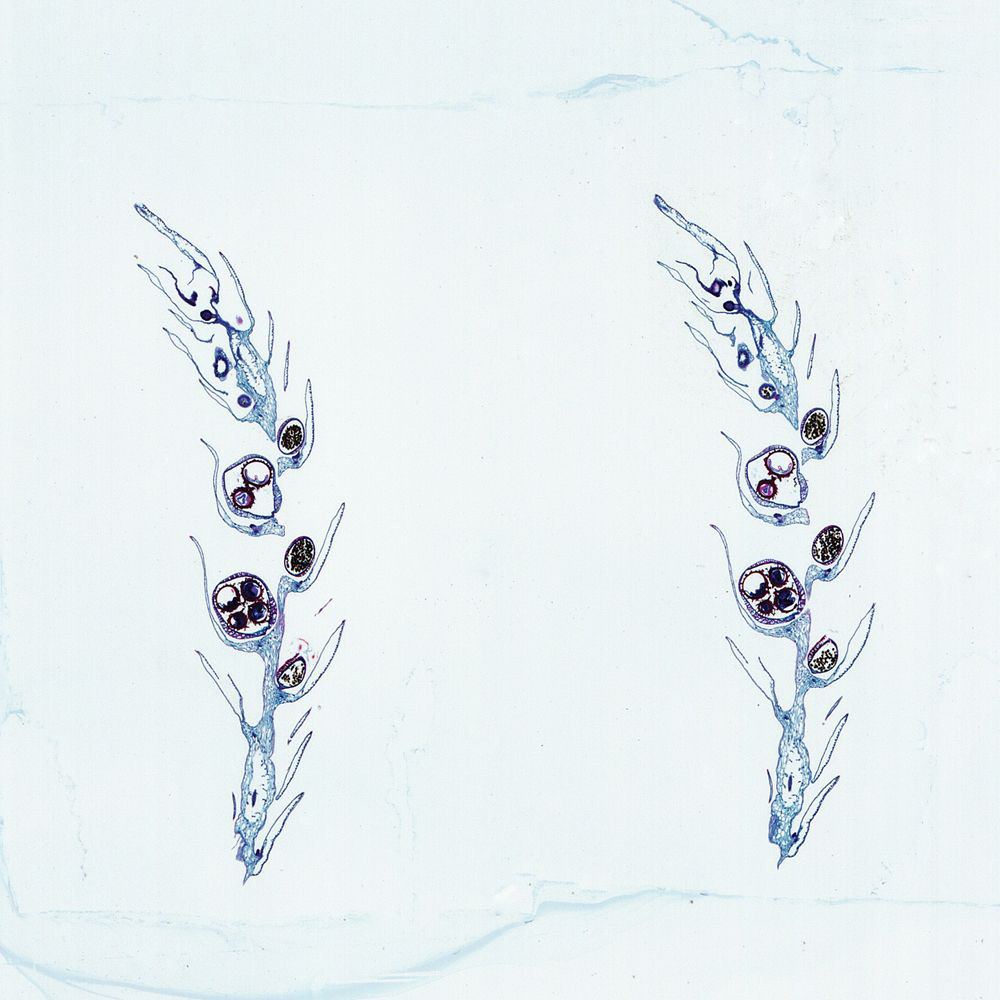
\includegraphics[width=0.7\linewidth]{./figures/mosses/selaginella_strobilus}

}

\caption{Selaginella strobilus.}\label{fig:selaginstrobilus}
\end{figure}

\section{Horsetails}\label{horsetails}

\href{https://en.wikipedia.org/wiki/Equisetum}{\emph{Equisetum}}
(horsetail) is the only living genus in Equisetaceae, a family of
vascular plants that reproduce by spores rather than seeds. \emph{Equisetum} is
a ``living fossil'' as it is the only living genus of the entire class
Equisetopsida, which for over one hundred million years was much more
diverse and dominated the understory of late Paleozoic forests. Some
Equisetopsida were large trees reaching to 30 meters tall.

\section{View Prepared Slides of
\emph{Equisetum}}\label{view-prepared-slides-of-equisetum}

\begin{enumerate}
\def\labelenumi{\arabic{enumi}.}
\tightlist
\item
  \emph{Equisetum} strobilus (Figure \ref{fig:equisetumstrobilus})

  \begin{itemize}
  \tightlist
  \item
    Identify: sporangiphores and spores
  \end{itemize}
\end{enumerate}

\begin{figure}

{\centering 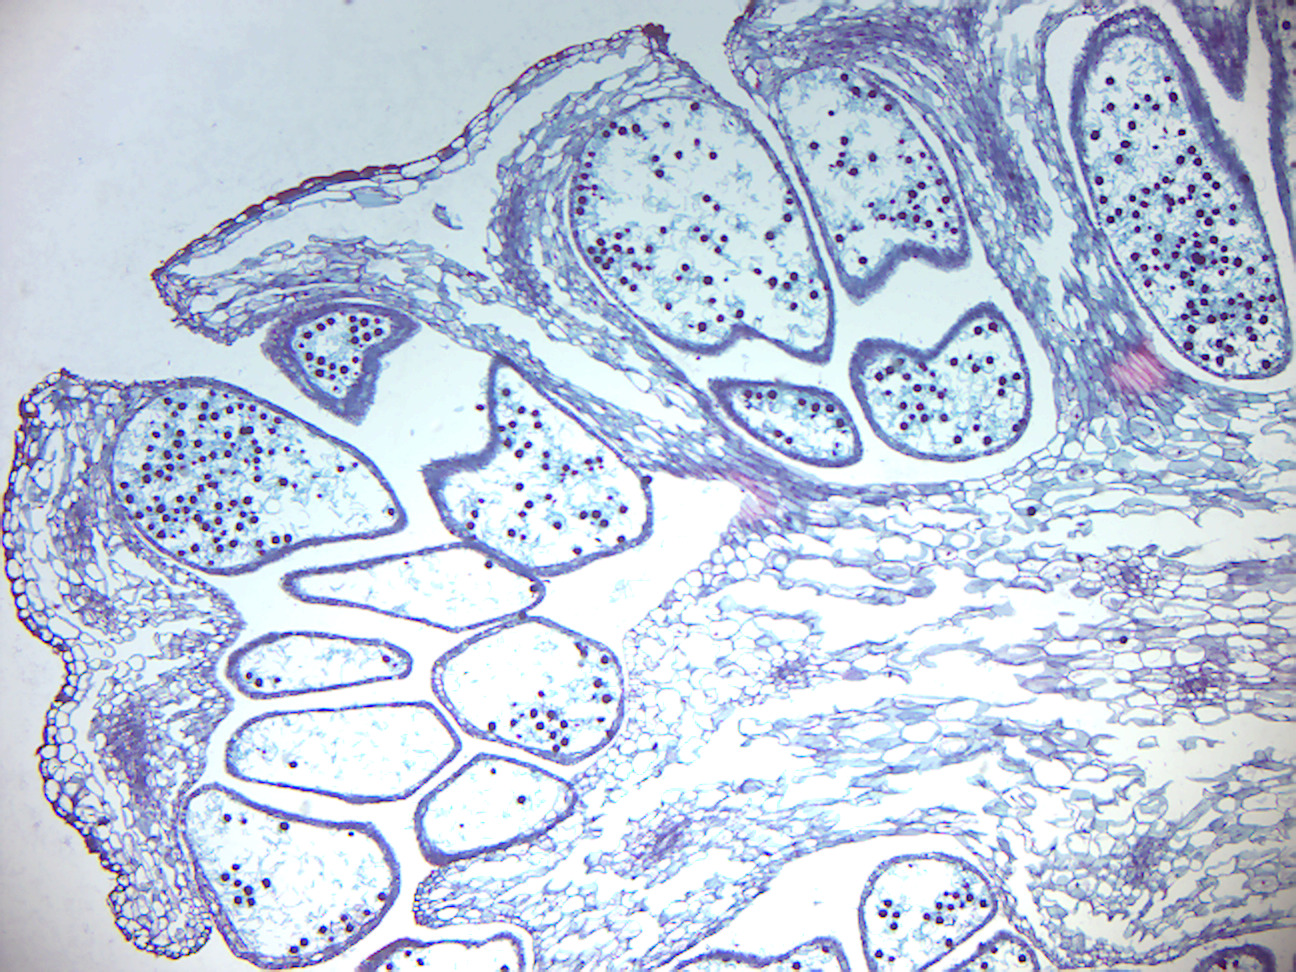
\includegraphics[width=0.7\linewidth]{./figures/mosses/equisetum_strobilus}

}

\caption{\emph{Equisetum} strobilus.}\label{fig:equisetumstrobilus}
\end{figure}

\section{Whisk ferns}\label{whisk-ferns}

\href{https://en.wikipedia.org/wiki/Psilotum}{\emph{Psilotum}} is a genus of
fern-like vascular plants, commonly known as whisk ferns. It is one of
two genera in the family Psilotaceae, the other being Tmesipteris. They
lack true roots and leaves, the stems being the organs containing
conducting tissue.

\section{View Prepared Slides of
\emph{Psilotum}}\label{view-prepared-slides-of-psilotum}

\begin{enumerate}
\def\labelenumi{\arabic{enumi}.}
\tightlist
\item
  \emph{Psilotum} sporangium (Figure \ref{fig:psilotumsporangium})

  \begin{itemize}
  \tightlist
  \item
    Identify: Sporangium, spores.
  \end{itemize}
\end{enumerate}

\begin{figure}

{\centering 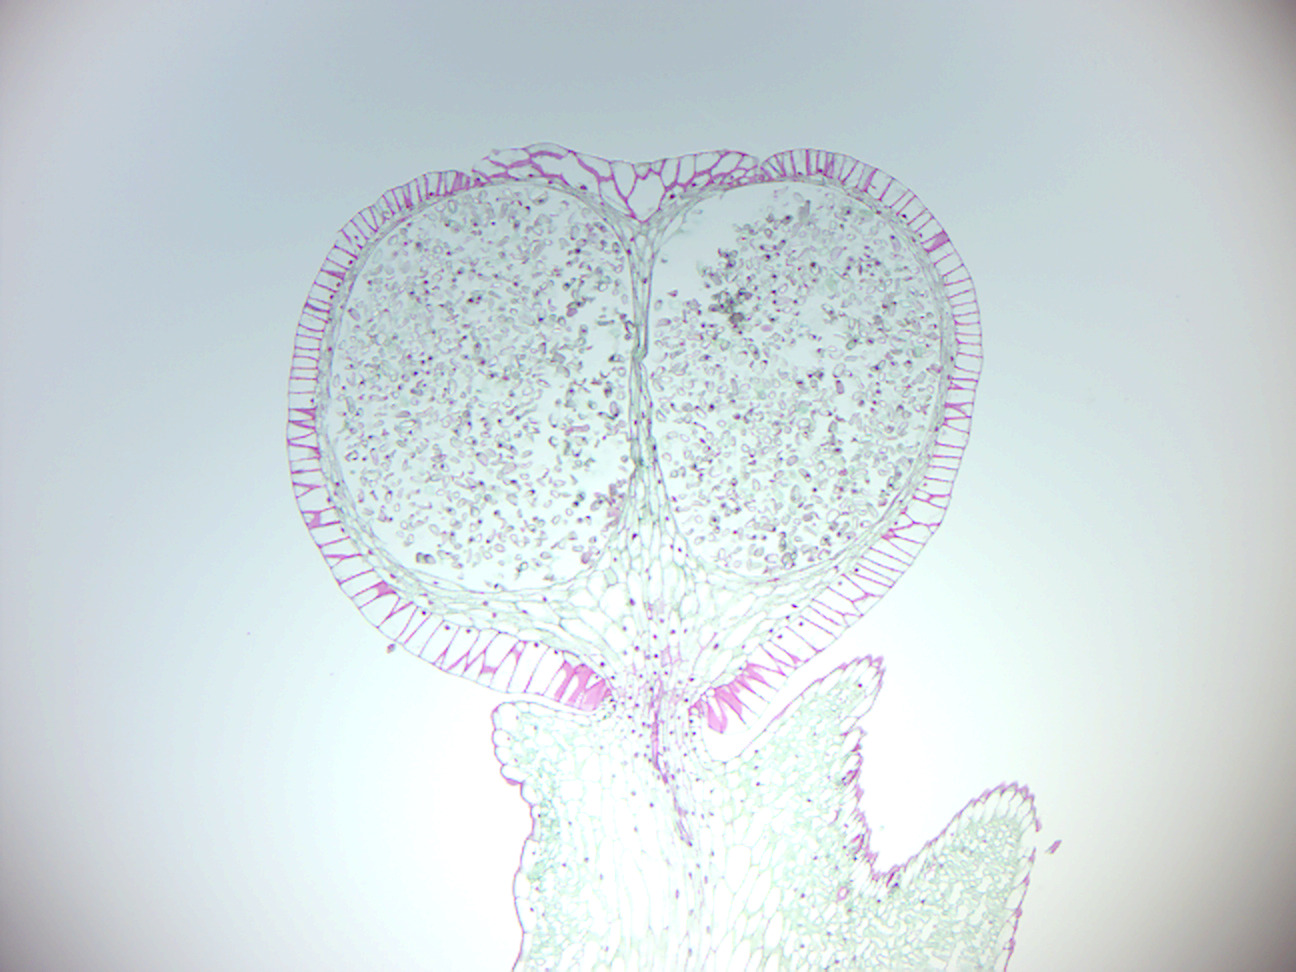
\includegraphics[width=0.7\linewidth]{./figures/mosses/psilotum_sporangium}

}

\caption{\emph{Psilotum} sporangium.}\label{fig:psilotumsporangium}
\end{figure}

\section{View Prepared Slides of
Ferns}\label{view-prepared-slides-of-ferns}

\begin{enumerate}
\def\labelenumi{\arabic{enumi}.}
\tightlist
\item
  Fern sporophyte (Figure \ref{fig:fernsporophyte})
\item
  Fern antheridia \& archegonia (Figure \ref{fig:ferngametophyte})

  \begin{itemize}
  \tightlist
  \item
    Identify: tissue of the gametophyte; antheridia; archegonia;
    rhizoids
  \end{itemize}
\item
  Fern prothallus young sporophyte (Figure \ref{fig:fernprothallus})

  \begin{itemize}
  \tightlist
  \item
    Identify: sporophyte, gametophyte; rhizoids
  \end{itemize}
\end{enumerate}

\begin{figure}

{\centering 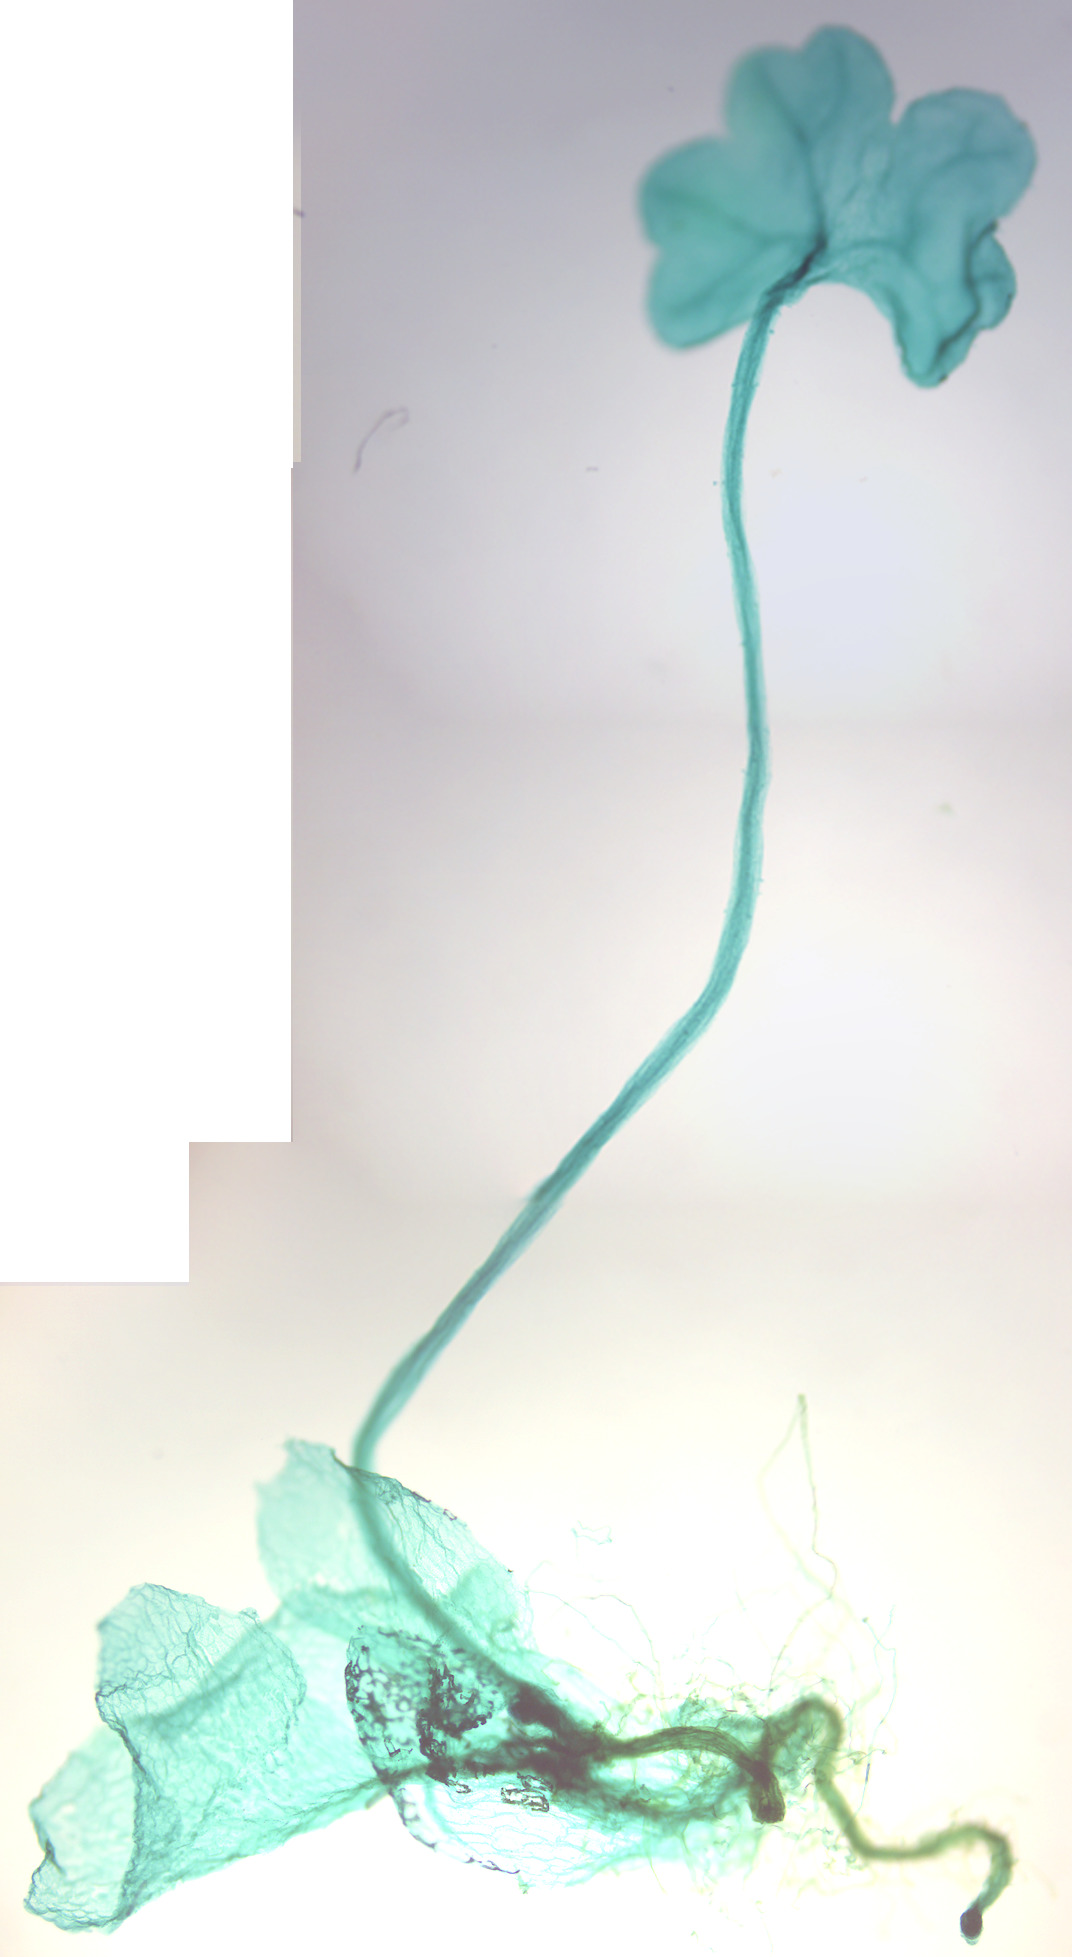
\includegraphics[width=0.7\linewidth]{./figures/mosses/fern_sporophyte}

}

\caption{Fern sporophyte.}\label{fig:fernsporophyte}
\end{figure}

\begin{figure}

{\centering 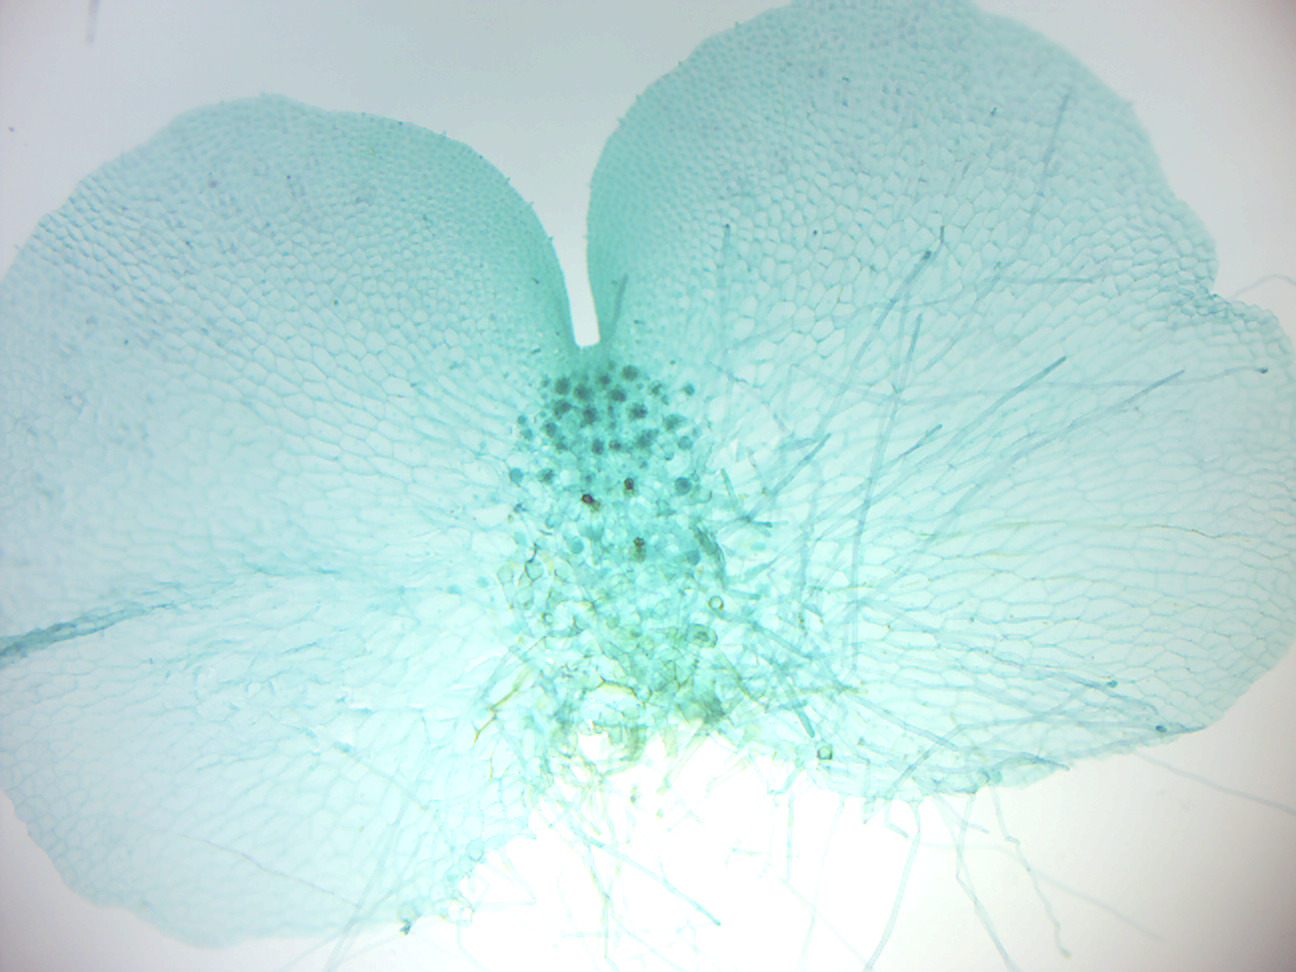
\includegraphics[width=0.7\linewidth]{./figures/mosses/fern_antheridia_archegonia}

}

\caption{Fern antheridia and archegonia.}\label{fig:ferngametophyte}
\end{figure}

\begin{figure}

{\centering 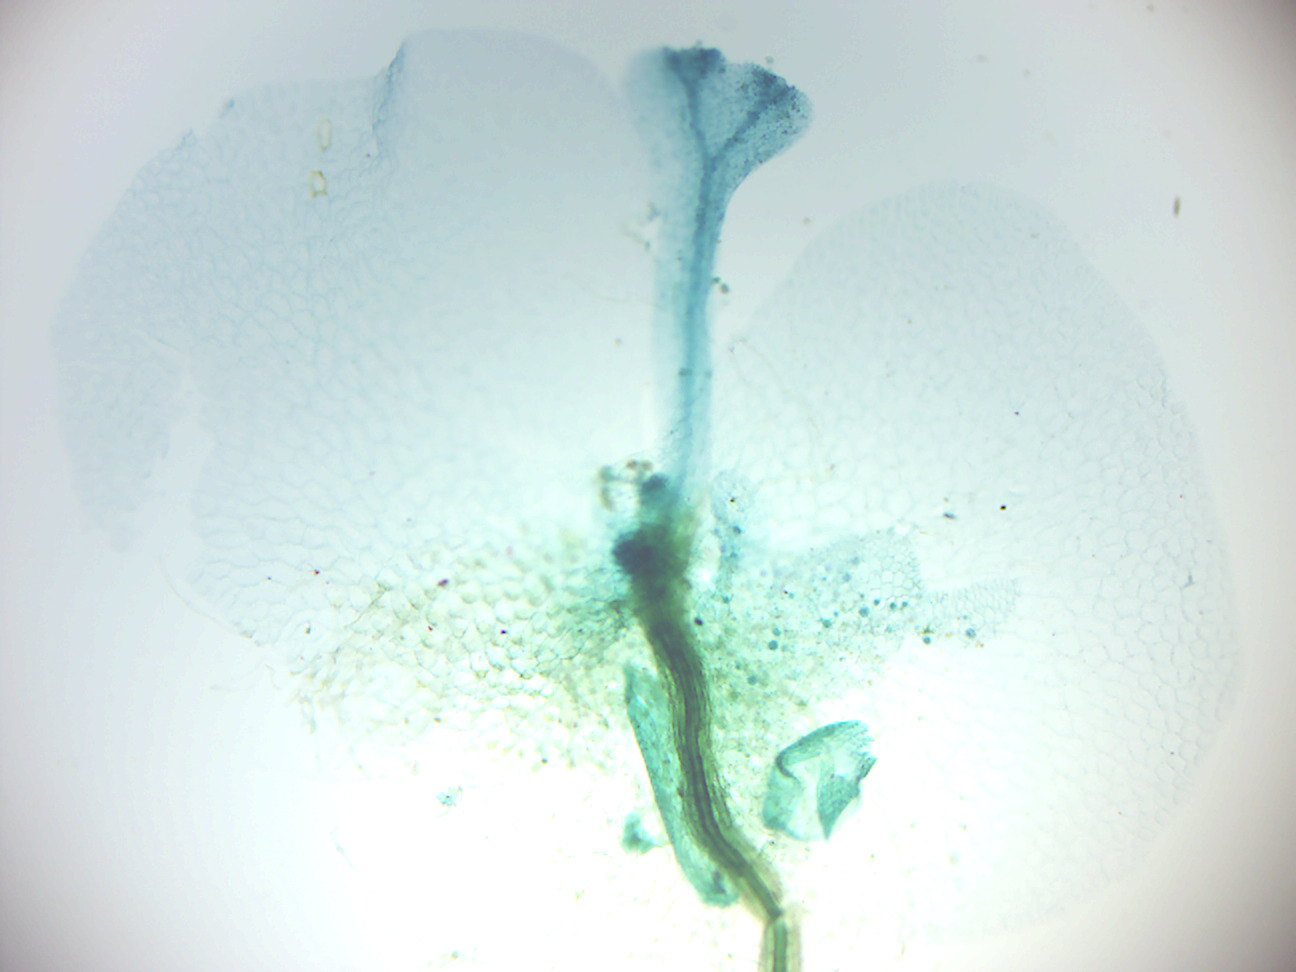
\includegraphics[width=0.7\linewidth]{./figures/mosses/fern_prothallus}

}

\caption{Fern prothallus young sporophyte.}\label{fig:fernprothallus}
\end{figure}

\section{View Prepared Slides of
\emph{Cyrtomium}}\label{view-prepared-slides-of-cyrtomium}

\href{https://en.wikipedia.org/wiki/Cyrtomium}{\emph{Cyrtomium}} is a
genus of about 15-20 species of ferns in the family Dryopteridaceae,
native to Asia, Africa (including Madagascar), and the Pacific Ocean
islands (Hawaii). \emph{Cyrtomium falcatum} is a species of fern known by the
common names house holly-fern and Japanese holly fern. It is native to
eastern Asia. It grows from crevices, coastal cliffs, streambanks, rocky
slopes, and other moist, stable areas.

\begin{enumerate}
\def\labelenumi{\arabic{enumi}.}
\tightlist
\item
  \emph{Cyrtomium falcatum} sorus on leaf

  \begin{itemize}
  \tightlist
  \item
    Locate sorus and identify the following: sporangia with spores
    inside; annular cells (annulus); lip cells; indusium (covering of
    the sorus).
  \end{itemize}
\end{enumerate}

\begin{figure}

{\centering 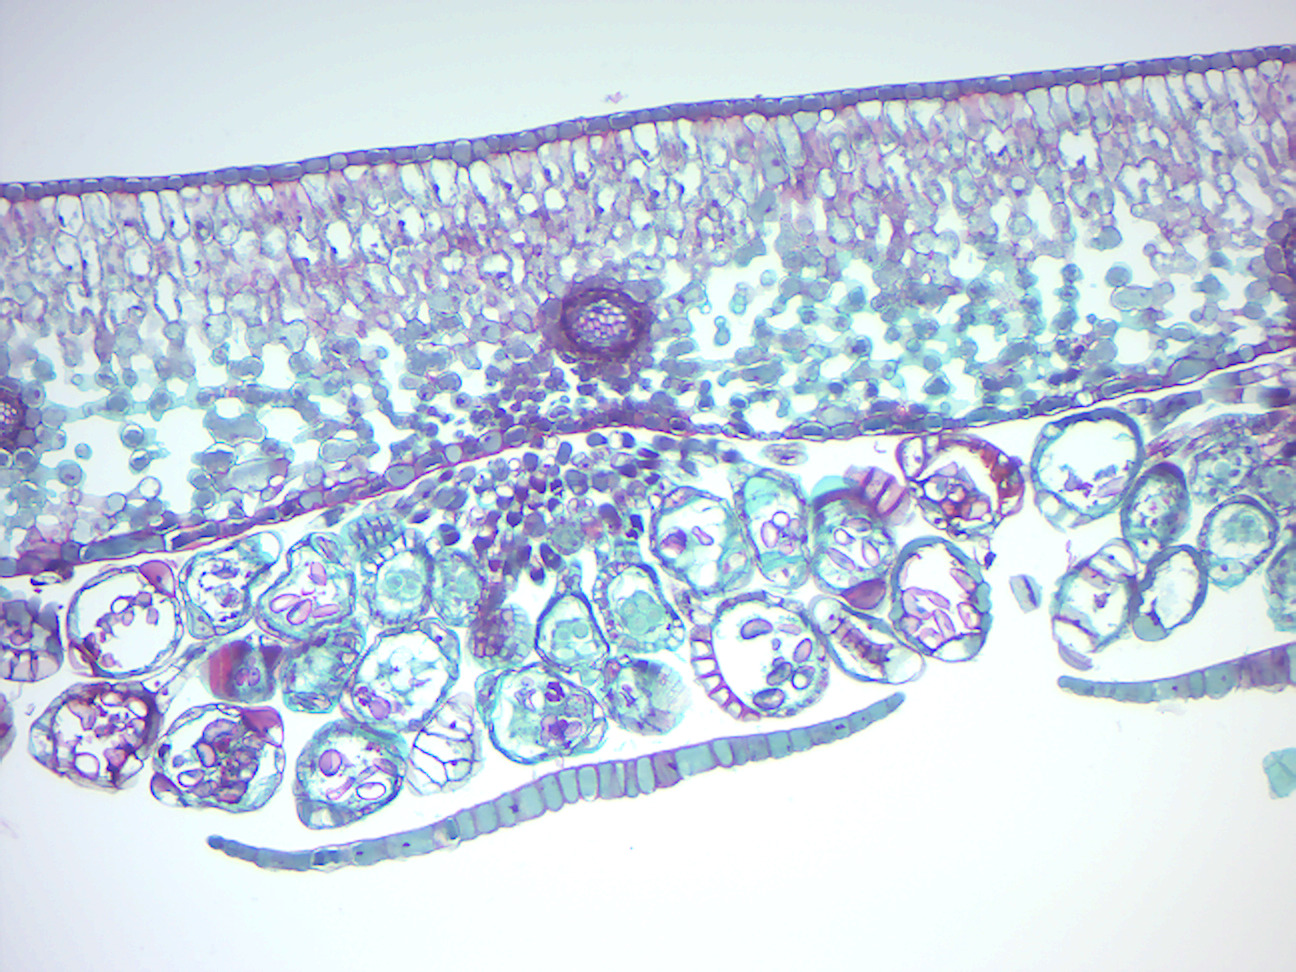
\includegraphics[width=0.7\linewidth]{./figures/mosses/cyrtomium_sorus}

}

\caption{\emph{Cyrtomium} falcatum sorus on leaf.}\label{fig:cyrtomium}
\end{figure}

\section{View Living Organisms}\label{view-living-organisms-1}

\begin{enumerate}
\def\labelenumi{\arabic{enumi}.}
\tightlist
\item
  Four types of Mosses
\item
  \emph{Marchantia hepatica}
\item
  \emph{Lycopodium lucidulum}
\end{enumerate}

\section{Review Questions}\label{review-questions-1}

\begin{enumerate}
\def\labelenumi{\arabic{enumi}.}
\tightlist
\item
  What are plants?
\item
  What are mosses?
\item
  What are liverworts?
\item
  What are ferns?
\item
  What does alternation of generations mean in the life cycle of plants?
\item
  What is a gametophyte?
\item
  What is a sporophyte?
\end{enumerate}
